\documentclass[twoside]{article}

% Packages required by doxygen
\usepackage{fixltx2e}
\usepackage{calc}
\usepackage{doxygen}
\usepackage[export]{adjustbox} % also loads graphicx
\usepackage{graphicx}
\usepackage[utf8]{inputenc}
\usepackage{makeidx}
\usepackage{multicol}
\usepackage{multirow}
\PassOptionsToPackage{warn}{textcomp}
\usepackage{textcomp}
\usepackage[nointegrals]{wasysym}
\usepackage[table]{xcolor}

% NLS support packages
\usepackage[T2A]{fontenc}
\usepackage[russian]{babel}

% Font selection
\usepackage[T1]{fontenc}
\usepackage[scaled=.90]{helvet}
\usepackage{courier}
\usepackage{amssymb}
\usepackage{sectsty}
\renewcommand{\familydefault}{\sfdefault}
\allsectionsfont{%
  \fontseries{bc}\selectfont%
  \color{darkgray}%
}
\renewcommand{\DoxyLabelFont}{%
  \fontseries{bc}\selectfont%
  \color{darkgray}%
}
\newcommand{\+}{\discretionary{\mbox{\scriptsize$\hookleftarrow$}}{}{}}

% Page & text layout
\usepackage{geometry}
\geometry{%
  a4paper,%
  top=2.5cm,%
  bottom=2.5cm,%
  left=2.5cm,%
  right=2.5cm%
}
\tolerance=750
\hfuzz=15pt
\hbadness=750
\setlength{\emergencystretch}{15pt}
\setlength{\parindent}{0cm}
\setlength{\parskip}{0.2cm}
\makeatletter
\renewcommand{\paragraph}{%
  \@startsection{paragraph}{4}{0ex}{-1.0ex}{1.0ex}{%
    \normalfont\normalsize\bfseries\SS@parafont%
  }%
}
\renewcommand{\subparagraph}{%
  \@startsection{subparagraph}{5}{0ex}{-1.0ex}{1.0ex}{%
    \normalfont\normalsize\bfseries\SS@subparafont%
  }%
}
\makeatother

% Headers & footers
\usepackage{fancyhdr}
\pagestyle{fancyplain}
\fancyhead[LE]{\fancyplain{}{\bfseries\thepage}}
\fancyhead[CE]{\fancyplain{}{}}
\fancyhead[RE]{\fancyplain{}{\bfseries\leftmark}}
\fancyhead[LO]{\fancyplain{}{\bfseries\rightmark}}
\fancyhead[CO]{\fancyplain{}{}}
\fancyhead[RO]{\fancyplain{}{\bfseries\thepage}}
\fancyfoot[LE]{\fancyplain{}{}}
\fancyfoot[CE]{\fancyplain{}{}}
\fancyfoot[RE]{\fancyplain{}{\bfseries\scriptsize Документация по mygrep. Последние изменения\+: Ср 18 Май 2016 04\+:38\+:18. Создано системой Doxygen }}
\fancyfoot[LO]{\fancyplain{}{\bfseries\scriptsize Документация по mygrep. Последние изменения\+: Ср 18 Май 2016 04\+:38\+:18. Создано системой Doxygen }}
\fancyfoot[CO]{\fancyplain{}{}}
\fancyfoot[RO]{\fancyplain{}{}}
\renewcommand{\footrulewidth}{0.4pt}
\renewcommand{\sectionmark}[1]{%
  \markright{\thesection\ #1}%
}

% Indices & bibliography
\usepackage{natbib}
\usepackage[titles]{tocloft}
\setcounter{tocdepth}{3}
\setcounter{secnumdepth}{5}
\makeindex

% Hyperlinks (required, but should be loaded last)
\usepackage{ifpdf}
\ifpdf
  \usepackage[pdftex,pagebackref=true]{hyperref}
\else
  \usepackage[ps2pdf,pagebackref=true]{hyperref}
\fi
\hypersetup{%
  colorlinks=true,%
  linkcolor=blue,%
  citecolor=blue,%
  unicode%
}

% Custom commands
\newcommand{\clearemptydoublepage}{%
  \newpage{\pagestyle{empty}\cleardoublepage}%
}


%===== C O N T E N T S =====

\begin{document}

% Titlepage & ToC
\hypersetup{pageanchor=false,
             bookmarks=true,
             bookmarksnumbered=true,
             pdfencoding=unicode
            }
\pagenumbering{roman}
\begin{titlepage}
\vspace*{7cm}
\begin{center}%
{\Large mygrep }\\
\vspace*{1cm}
{\large Создано системой Doxygen 1.8.10}\\
\vspace*{0.5cm}
{\small Ср 18 Май 2016 04:38:18}\\
\end{center}
\end{titlepage}
\tableofcontents
\pagenumbering{arabic}
\hypersetup{pageanchor=true}

%--- Begin generated contents ---
\section{mygrep}
\label{index}\hypertarget{index}{}\begin{DoxyAuthor}{Автор}
Антон Ханджян, 205 группа ВМК МГУ 
\end{DoxyAuthor}

\section{Алфавитный указатель классов}
\subsection{Классы}
Классы с их кратким описанием.\begin{DoxyCompactList}
\item\contentsline{section}{\hyperlink{class_lex}{Lex} \\*Лексический анализатор }{\pageref{class_lex}}{}
\item\contentsline{section}{\hyperlink{class_lexem}{Lexem} \\*Класс лексем }{\pageref{class_lexem}}{}
\item\contentsline{section}{\hyperlink{class_mygrep}{Mygrep} \\*Обработчик регулярных выражений }{\pageref{class_mygrep}}{}
\item\contentsline{section}{\hyperlink{class_syn__lexem}{Syn\+\_\+lexem} \\*Синтаксические лексемы }{\pageref{class_syn__lexem}}{}
\item\contentsline{section}{\hyperlink{class_syntax}{Syntax} \\*Синтаксический анализатор }{\pageref{class_syntax}}{}
\end{DoxyCompactList}

\section{Список файлов}
\subsection{Файлы}
Полный список документированных файлов.\begin{DoxyCompactList}
\item\contentsline{section}{\hyperlink{lexic_8cpp}{lexic.\+cpp} \\*Файл с реализацией лексического анализатора }{\pageref{lexic_8cpp}}{}
\item\contentsline{section}{\hyperlink{lexic_8h}{lexic.\+h} \\*Заголовочный файл лексического анализатора }{\pageref{lexic_8h}}{}
\item\contentsline{section}{\hyperlink{mygrep_8cpp}{mygrep.\+cpp} \\*Файл с реализацией основного функционала программы }{\pageref{mygrep_8cpp}}{}
\item\contentsline{section}{\hyperlink{mygrep_8h}{mygrep.\+h} \\*Заголовочный файл пользовательськой части программы }{\pageref{mygrep_8h}}{}
\item\contentsline{section}{\hyperlink{syntax_8cpp}{syntax.\+cpp} \\*Файл с реализацией синтаксического анализатора }{\pageref{syntax_8cpp}}{}
\item\contentsline{section}{\hyperlink{syntax_8h}{syntax.\+h} \\*Заголовочный файл синтаксического анализатора }{\pageref{syntax_8h}}{}
\end{DoxyCompactList}

\section{Классы}
\hypertarget{class_lex}{}\subsection{Класс Lex}
\label{class_lex}\index{Lex@{Lex}}


Лексический анализатор  




{\ttfamily \#include $<$lexic.\+h$>$}

\subsubsection*{Закрытые члены}
\begin{DoxyCompactItemize}
\item 
bool \hyperlink{class_lex_a3b9276570c7b49bb53f646419fdc1cbf}{isoper} (char ch)
\begin{DoxyCompactList}\small\item\em Функция, проверяющая является ли символ оператором \end{DoxyCompactList}\item 
bool \hyperlink{class_lex_a8649a6722fbdc0eb2b331901e959e2d6}{isterm} (char ch)
\begin{DoxyCompactList}\small\item\em Функция, проверяющая является ли символ терминальным \end{DoxyCompactList}\item 
\hyperlink{class_lex_a2d9cafe03428afbced68bb4581357114}{Lex} (const string \&reg)
\begin{DoxyCompactList}\small\item\em Конструктор от строки с регулярным выражением. \end{DoxyCompactList}\item 
\hyperlink{class_lexem}{Lexem} \hyperlink{class_lex_a38b6e95d1a98fd656ee932d34018a0aa}{get\+\_\+lex} ()
\begin{DoxyCompactList}\small\item\em Функция, последовательно возвращающая лексемы \end{DoxyCompactList}\end{DoxyCompactItemize}
\subsubsection*{Закрытые данные}
\begin{DoxyCompactItemize}
\item 
\hypertarget{class_lex_a1a29de7eb28089a8d88922fc06ad322d}{}vector$<$ \hyperlink{class_lexem}{Lexem} $>$ \hyperlink{class_lex_a1a29de7eb28089a8d88922fc06ad322d}{lexems}\label{class_lex_a1a29de7eb28089a8d88922fc06ad322d}

\begin{DoxyCompactList}\small\item\em Вектор, в который записывается последовательность лексем, эквивалентная исходному регулярному выражению \end{DoxyCompactList}\item 
\hypertarget{class_lex_ab6d830f1859bbb9a6d18ba0751f43255}{}unsigned \hyperlink{class_lex_ab6d830f1859bbb9a6d18ba0751f43255}{cur} = 0\label{class_lex_ab6d830f1859bbb9a6d18ba0751f43255}

\begin{DoxyCompactList}\small\item\em Текущая позиция в векторе lexems (для функции \hyperlink{class_lex_a38b6e95d1a98fd656ee932d34018a0aa}{get\+\_\+lex()}) \end{DoxyCompactList}\end{DoxyCompactItemize}
\subsubsection*{Закрытые статические данные}
\begin{DoxyCompactItemize}
\item 
static char \hyperlink{class_lex_ad87b6f7104bb60dee3cf0c196b5b46cd}{possible\+\_\+op} \mbox{[}$\,$\mbox{]}
\begin{DoxyCompactList}\small\item\em служебный массив символов, имеющих значение операций \end{DoxyCompactList}\end{DoxyCompactItemize}
\subsubsection*{Друзья}
\begin{DoxyCompactItemize}
\item 
\hypertarget{class_lex_a13fb68a36cac69480f7fd4b3900594f9}{}class {\bfseries Syntax}\label{class_lex_a13fb68a36cac69480f7fd4b3900594f9}

\end{DoxyCompactItemize}


\subsubsection{Подробное описание}
Лексический анализатор 

Лексический анализатор преобразует исходную строку в последовательность типизированных лексем и проверяет правильность экранирования символов и написания многосимвольных операторов 

\subsubsection{Конструктор(ы)}
\hypertarget{class_lex_a2d9cafe03428afbced68bb4581357114}{}\index{Lex@{Lex}!Lex@{Lex}}
\index{Lex@{Lex}!Lex@{Lex}}
\paragraph[{Lex(const string \&reg)}]{\setlength{\rightskip}{0pt plus 5cm}Lex\+::\+Lex (
\begin{DoxyParamCaption}
\item[{const string \&}]{reg}
\end{DoxyParamCaption}
)\hspace{0.3cm}{\ttfamily [explicit]}, {\ttfamily [private]}}\label{class_lex_a2d9cafe03428afbced68bb4581357114}


Конструктор от строки с регулярным выражением. 

Сделан явным, поскольку неясен смысл выражения вида \hyperlink{class_lex}{Lex} c = \char`\"{}a$\ast$\char`\"{}; 

Граф вызовов\+:
\nopagebreak
\begin{figure}[H]
\begin{center}
\leavevmode
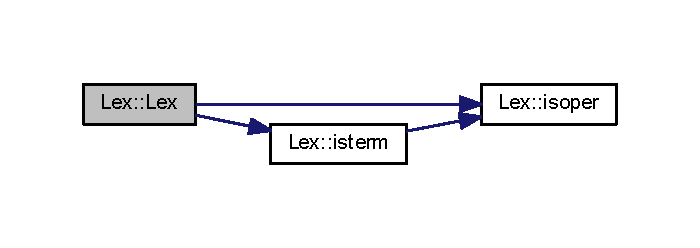
\includegraphics[width=336pt]{class_lex_a2d9cafe03428afbced68bb4581357114_cgraph}
\end{center}
\end{figure}




\subsubsection{Методы}
\hypertarget{class_lex_a38b6e95d1a98fd656ee932d34018a0aa}{}\index{Lex@{Lex}!get\+\_\+lex@{get\+\_\+lex}}
\index{get\+\_\+lex@{get\+\_\+lex}!Lex@{Lex}}
\paragraph[{get\+\_\+lex()}]{\setlength{\rightskip}{0pt plus 5cm}{\bf Lexem} Lex\+::get\+\_\+lex (
\begin{DoxyParamCaption}
{}
\end{DoxyParamCaption}
)\hspace{0.3cm}{\ttfamily [private]}}\label{class_lex_a38b6e95d1a98fd656ee932d34018a0aa}


Функция, последовательно возвращающая лексемы 

\begin{DoxyReturn}{Возвращает}
Возвращает очередную лексему 
\end{DoxyReturn}
\hypertarget{class_lex_a3b9276570c7b49bb53f646419fdc1cbf}{}\index{Lex@{Lex}!isoper@{isoper}}
\index{isoper@{isoper}!Lex@{Lex}}
\paragraph[{isoper(char ch)}]{\setlength{\rightskip}{0pt plus 5cm}bool Lex\+::isoper (
\begin{DoxyParamCaption}
\item[{char}]{ch}
\end{DoxyParamCaption}
)\hspace{0.3cm}{\ttfamily [private]}}\label{class_lex_a3b9276570c7b49bb53f646419fdc1cbf}


Функция, проверяющая является ли символ оператором 


\begin{DoxyParams}[1]{Аргументы}
\mbox{\tt in}  & {\em ch} & Символ для проверки \\
\hline
\end{DoxyParams}
\begin{DoxyReturn}{Возвращает}
true, если символ является оператором, false — иначе 
\end{DoxyReturn}
\hypertarget{class_lex_a8649a6722fbdc0eb2b331901e959e2d6}{}\index{Lex@{Lex}!isterm@{isterm}}
\index{isterm@{isterm}!Lex@{Lex}}
\paragraph[{isterm(char ch)}]{\setlength{\rightskip}{0pt plus 5cm}bool Lex\+::isterm (
\begin{DoxyParamCaption}
\item[{char}]{ch}
\end{DoxyParamCaption}
)\hspace{0.3cm}{\ttfamily [private]}}\label{class_lex_a8649a6722fbdc0eb2b331901e959e2d6}


Функция, проверяющая является ли символ терминальным 


\begin{DoxyParams}[1]{Аргументы}
\mbox{\tt in}  & {\em ch} & Символ для проверки \\
\hline
\end{DoxyParams}
\begin{DoxyReturn}{Возвращает}
{\bfseries true}, если символ является терминальным, false — иначе 
\end{DoxyReturn}


Граф вызовов\+:
\nopagebreak
\begin{figure}[H]
\begin{center}
\leavevmode
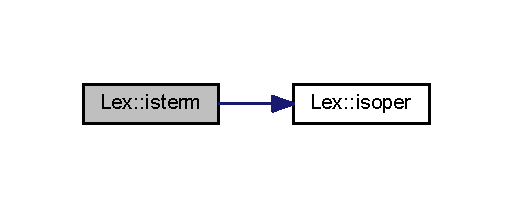
\includegraphics[width=246pt]{class_lex_a8649a6722fbdc0eb2b331901e959e2d6_cgraph}
\end{center}
\end{figure}




\subsubsection{Данные класса}
\hypertarget{class_lex_ad87b6f7104bb60dee3cf0c196b5b46cd}{}\index{Lex@{Lex}!possible\+\_\+op@{possible\+\_\+op}}
\index{possible\+\_\+op@{possible\+\_\+op}!Lex@{Lex}}
\paragraph[{possible\+\_\+op}]{\setlength{\rightskip}{0pt plus 5cm}char Lex\+::possible\+\_\+op\hspace{0.3cm}{\ttfamily [static]}, {\ttfamily [private]}}\label{class_lex_ad87b6f7104bb60dee3cf0c196b5b46cd}
{\bfseries Инициализатор}
\begin{DoxyCode}
=
\{
    \textcolor{charliteral}{'*'},
    \textcolor{charliteral}{'|'},
    \textcolor{charliteral}{'('},
    \textcolor{charliteral}{')'},
    \textcolor{charliteral}{'+'},
    \textcolor{charliteral}{'?'},
    \textcolor{charliteral}{'\{'},
    \textcolor{charliteral}{'\}'},
    \textcolor{charliteral}{'['},
    \textcolor{charliteral}{']'},
    \textcolor{charliteral}{'-'},
    \textcolor{charliteral}{'\(\backslash\)\(\backslash\)'},
    0
\}
\end{DoxyCode}


служебный массив символов, имеющих значение операций 



Объявления и описания членов классов находятся в файлах\+:\begin{DoxyCompactItemize}
\item 
\hyperlink{lexic_8h}{lexic.\+h}\item 
\hyperlink{lexic_8cpp}{lexic.\+cpp}\end{DoxyCompactItemize}

\hypertarget{class_lexem}{}\subsection{Класс Lexem}
\label{class_lexem}\index{Lexem@{Lexem}}


Класс лексем  




{\ttfamily \#include $<$lexic.\+h$>$}

\subsubsection*{Закрытые типы}
\begin{DoxyCompactItemize}
\item 
enum \hyperlink{class_lexem_af335177220e991d190a36fabef7ecbf4}{lexem\+\_\+types} \{ \\*
\hyperlink{class_lexem_af335177220e991d190a36fabef7ecbf4a0c2b508143050096f01e47223d7b656e}{O\+P\+E\+N\+\_\+\+B\+R\+A\+C\+E}, 
\hyperlink{class_lexem_af335177220e991d190a36fabef7ecbf4a459f9d21f9a7fd564322ff78846d6c55}{C\+L\+O\+S\+E\+\_\+\+B\+R\+A\+C\+E}, 
\hyperlink{class_lexem_af335177220e991d190a36fabef7ecbf4a84aae9f4818d90bf027d51e43fdf2104}{I\+T\+E\+R}, 
\hyperlink{class_lexem_af335177220e991d190a36fabef7ecbf4a233bedb05d38fbfb1176d2f662f86787}{I\+T\+E\+R\+\_\+\+N\+\_\+\+M}, 
\\*
\hyperlink{class_lexem_af335177220e991d190a36fabef7ecbf4a9fa4026ec33d2580f220ff6b8cdae2fb}{L\+A\+Z\+Y\+\_\+\+I\+T\+E\+R}, 
\hyperlink{class_lexem_af335177220e991d190a36fabef7ecbf4aa942c8254c90bee7ec5588a318b84022}{T\+E\+R\+M\+I\+N\+A\+L}, 
\hyperlink{class_lexem_af335177220e991d190a36fabef7ecbf4a629e010881951d564f7bb217dacb0b74}{O\+R}, 
\hyperlink{class_lexem_af335177220e991d190a36fabef7ecbf4a45577586a792f3738569d22ff9192976}{E\+N\+D}
 \}\begin{DoxyCompactList}\small\item\em Возможные типы лексем \end{DoxyCompactList}
\end{DoxyCompactItemize}
\subsubsection*{Закрытые члены}
\begin{DoxyCompactItemize}
\item 
\hyperlink{class_lexem_a707b1ec3c3640fb40e8ac69e7b0aac63}{Lexem} (\hyperlink{class_lexem_af335177220e991d190a36fabef7ecbf4}{lexem\+\_\+types} \hyperlink{class_lexem_ad60447d5e5f83d8c95d3f658930ab13d}{type}=\hyperlink{class_lexem_af335177220e991d190a36fabef7ecbf4a45577586a792f3738569d22ff9192976}{E\+N\+D}, int \hyperlink{class_lexem_af0a7790d19219952191379409afa505e}{param1}=0, int \hyperlink{class_lexem_a2a89063a544c399b2dfc9a775e94b13b}{param2}=0)
\item 
\hyperlink{class_lexem_a8c81179e58f3d67b43fb92959dec0476}{Lexem} (string \&\hyperlink{class_lexem_a2d5cea0d9f7cbaf5edd5973991d0da7a}{terminal})
\item 
\hypertarget{class_lexem_ab863374b860c4eb4c150ddb8748a206d}{}void \hyperlink{class_lexem_ab863374b860c4eb4c150ddb8748a206d}{print} ()\label{class_lexem_ab863374b860c4eb4c150ddb8748a206d}

\begin{DoxyCompactList}\small\item\em Функция распечатывает лексемы в исходном виде \end{DoxyCompactList}\end{DoxyCompactItemize}
\subsubsection*{Закрытые данные}
\begin{DoxyCompactItemize}
\item 
\hypertarget{class_lexem_a2d5cea0d9f7cbaf5edd5973991d0da7a}{}string \hyperlink{class_lexem_a2d5cea0d9f7cbaf5edd5973991d0da7a}{terminal} = \char`\"{}\char`\"{}\label{class_lexem_a2d5cea0d9f7cbaf5edd5973991d0da7a}

\begin{DoxyCompactList}\small\item\em Терминальная цепочка \end{DoxyCompactList}\item 
\hypertarget{class_lexem_af0a7790d19219952191379409afa505e}{}int \hyperlink{class_lexem_af0a7790d19219952191379409afa505e}{param1} = 0\label{class_lexem_af0a7790d19219952191379409afa505e}

\begin{DoxyCompactList}\small\item\em Первый параметр лексемы \end{DoxyCompactList}\item 
\hypertarget{class_lexem_a2a89063a544c399b2dfc9a775e94b13b}{}int \hyperlink{class_lexem_a2a89063a544c399b2dfc9a775e94b13b}{param2} = 0\label{class_lexem_a2a89063a544c399b2dfc9a775e94b13b}

\begin{DoxyCompactList}\small\item\em Второй параметр лексемы \end{DoxyCompactList}\item 
\hypertarget{class_lexem_ad60447d5e5f83d8c95d3f658930ab13d}{}\hyperlink{class_lexem_af335177220e991d190a36fabef7ecbf4}{lexem\+\_\+types} \hyperlink{class_lexem_ad60447d5e5f83d8c95d3f658930ab13d}{type}\label{class_lexem_ad60447d5e5f83d8c95d3f658930ab13d}

\begin{DoxyCompactList}\small\item\em Тип лексемы \end{DoxyCompactList}\end{DoxyCompactItemize}
\subsubsection*{Друзья}
\begin{DoxyCompactItemize}
\item 
\hypertarget{class_lexem_a90fdb1ff12233c504810e346b5f6e49f}{}class {\bfseries Mygrep}\label{class_lexem_a90fdb1ff12233c504810e346b5f6e49f}

\item 
\hypertarget{class_lexem_a13fb68a36cac69480f7fd4b3900594f9}{}class {\bfseries Syntax}\label{class_lexem_a13fb68a36cac69480f7fd4b3900594f9}

\item 
\hypertarget{class_lexem_a1bd3ddc25649d03c17431b42bd4ad50d}{}class {\bfseries Lex}\label{class_lexem_a1bd3ddc25649d03c17431b42bd4ad50d}

\item 
\hypertarget{class_lexem_a8b6b352adcaf7ac2805f59bb6204794e}{}class {\bfseries Syn\+\_\+lexem}\label{class_lexem_a8b6b352adcaf7ac2805f59bb6204794e}

\end{DoxyCompactItemize}


\subsubsection{Подробное описание}
Класс лексем 

\subsubsection{Перечисления}
\hypertarget{class_lexem_af335177220e991d190a36fabef7ecbf4}{}\index{Lexem@{Lexem}!lexem\+\_\+types@{lexem\+\_\+types}}
\index{lexem\+\_\+types@{lexem\+\_\+types}!Lexem@{Lexem}}
\paragraph[{lexem\+\_\+types}]{\setlength{\rightskip}{0pt plus 5cm}enum {\bf Lexem\+::lexem\+\_\+types}\hspace{0.3cm}{\ttfamily [private]}}\label{class_lexem_af335177220e991d190a36fabef7ecbf4}


Возможные типы лексем 

\begin{Desc}
\item[Элементы перечислений]\par
\begin{description}
\index{O\+P\+E\+N\+\_\+\+B\+R\+A\+C\+E@{O\+P\+E\+N\+\_\+\+B\+R\+A\+C\+E}!Lexem@{Lexem}}\index{Lexem@{Lexem}!O\+P\+E\+N\+\_\+\+B\+R\+A\+C\+E@{O\+P\+E\+N\+\_\+\+B\+R\+A\+C\+E}}\item[{\em 
\hypertarget{class_lexem_af335177220e991d190a36fabef7ecbf4a0c2b508143050096f01e47223d7b656e}{}O\+P\+E\+N\+\_\+\+B\+R\+A\+C\+E\label{class_lexem_af335177220e991d190a36fabef7ecbf4a0c2b508143050096f01e47223d7b656e}
}]Открывающая скобка \index{C\+L\+O\+S\+E\+\_\+\+B\+R\+A\+C\+E@{C\+L\+O\+S\+E\+\_\+\+B\+R\+A\+C\+E}!Lexem@{Lexem}}\index{Lexem@{Lexem}!C\+L\+O\+S\+E\+\_\+\+B\+R\+A\+C\+E@{C\+L\+O\+S\+E\+\_\+\+B\+R\+A\+C\+E}}\item[{\em 
\hypertarget{class_lexem_af335177220e991d190a36fabef7ecbf4a459f9d21f9a7fd564322ff78846d6c55}{}C\+L\+O\+S\+E\+\_\+\+B\+R\+A\+C\+E\label{class_lexem_af335177220e991d190a36fabef7ecbf4a459f9d21f9a7fd564322ff78846d6c55}
}]Закрывающая скобка \index{I\+T\+E\+R@{I\+T\+E\+R}!Lexem@{Lexem}}\index{Lexem@{Lexem}!I\+T\+E\+R@{I\+T\+E\+R}}\item[{\em 
\hypertarget{class_lexem_af335177220e991d190a36fabef7ecbf4a84aae9f4818d90bf027d51e43fdf2104}{}I\+T\+E\+R\label{class_lexem_af335177220e991d190a36fabef7ecbf4a84aae9f4818d90bf027d51e43fdf2104}
}]Итерация \index{I\+T\+E\+R\+\_\+\+N\+\_\+\+M@{I\+T\+E\+R\+\_\+\+N\+\_\+\+M}!Lexem@{Lexem}}\index{Lexem@{Lexem}!I\+T\+E\+R\+\_\+\+N\+\_\+\+M@{I\+T\+E\+R\+\_\+\+N\+\_\+\+M}}\item[{\em 
\hypertarget{class_lexem_af335177220e991d190a36fabef7ecbf4a233bedb05d38fbfb1176d2f662f86787}{}I\+T\+E\+R\+\_\+\+N\+\_\+\+M\label{class_lexem_af335177220e991d190a36fabef7ecbf4a233bedb05d38fbfb1176d2f662f86787}
}]Итерация от n до m раз \index{L\+A\+Z\+Y\+\_\+\+I\+T\+E\+R@{L\+A\+Z\+Y\+\_\+\+I\+T\+E\+R}!Lexem@{Lexem}}\index{Lexem@{Lexem}!L\+A\+Z\+Y\+\_\+\+I\+T\+E\+R@{L\+A\+Z\+Y\+\_\+\+I\+T\+E\+R}}\item[{\em 
\hypertarget{class_lexem_af335177220e991d190a36fabef7ecbf4a9fa4026ec33d2580f220ff6b8cdae2fb}{}L\+A\+Z\+Y\+\_\+\+I\+T\+E\+R\label{class_lexem_af335177220e991d190a36fabef7ecbf4a9fa4026ec33d2580f220ff6b8cdae2fb}
}]Ленивая итерация \index{T\+E\+R\+M\+I\+N\+A\+L@{T\+E\+R\+M\+I\+N\+A\+L}!Lexem@{Lexem}}\index{Lexem@{Lexem}!T\+E\+R\+M\+I\+N\+A\+L@{T\+E\+R\+M\+I\+N\+A\+L}}\item[{\em 
\hypertarget{class_lexem_af335177220e991d190a36fabef7ecbf4aa942c8254c90bee7ec5588a318b84022}{}T\+E\+R\+M\+I\+N\+A\+L\label{class_lexem_af335177220e991d190a36fabef7ecbf4aa942c8254c90bee7ec5588a318b84022}
}]Терминальная цепочка \index{O\+R@{O\+R}!Lexem@{Lexem}}\index{Lexem@{Lexem}!O\+R@{O\+R}}\item[{\em 
\hypertarget{class_lexem_af335177220e991d190a36fabef7ecbf4a629e010881951d564f7bb217dacb0b74}{}O\+R\label{class_lexem_af335177220e991d190a36fabef7ecbf4a629e010881951d564f7bb217dacb0b74}
}]Перечисление \index{E\+N\+D@{E\+N\+D}!Lexem@{Lexem}}\index{Lexem@{Lexem}!E\+N\+D@{E\+N\+D}}\item[{\em 
\hypertarget{class_lexem_af335177220e991d190a36fabef7ecbf4a45577586a792f3738569d22ff9192976}{}E\+N\+D\label{class_lexem_af335177220e991d190a36fabef7ecbf4a45577586a792f3738569d22ff9192976}
}]Признак конца \end{description}
\end{Desc}


\subsubsection{Конструктор(ы)}
\hypertarget{class_lexem_a707b1ec3c3640fb40e8ac69e7b0aac63}{}\index{Lexem@{Lexem}!Lexem@{Lexem}}
\index{Lexem@{Lexem}!Lexem@{Lexem}}
\paragraph[{Lexem(lexem\+\_\+types type=\+E\+N\+D, int param1=0, int param2=0)}]{\setlength{\rightskip}{0pt plus 5cm}Lexem\+::\+Lexem (
\begin{DoxyParamCaption}
\item[{{\bf lexem\+\_\+types}}]{type = {\ttfamily {\bf E\+N\+D}}, }
\item[{int}]{param1 = {\ttfamily 0}, }
\item[{int}]{param2 = {\ttfamily 0}}
\end{DoxyParamCaption}
)\hspace{0.3cm}{\ttfamily [inline]}, {\ttfamily [private]}}\label{class_lexem_a707b1ec3c3640fb40e8ac69e7b0aac63}
Конструктор для нетерминальной лексемы 
\begin{DoxyParams}[1]{Аргументы}
\mbox{\tt in}  & {\em type} & Тип лексемы. По умолчанию E\+N\+D \\
\hline
\mbox{\tt in}  & {\em param1} & Первый параметр лексемы. По умолчанию 0 \\
\hline
\mbox{\tt in}  & {\em param1} & Второй параметр лексемы. По умолчанию 0 \\
\hline
\end{DoxyParams}
\hypertarget{class_lexem_a8c81179e58f3d67b43fb92959dec0476}{}\index{Lexem@{Lexem}!Lexem@{Lexem}}
\index{Lexem@{Lexem}!Lexem@{Lexem}}
\paragraph[{Lexem(string \&terminal)}]{\setlength{\rightskip}{0pt plus 5cm}Lexem\+::\+Lexem (
\begin{DoxyParamCaption}
\item[{string \&}]{terminal}
\end{DoxyParamCaption}
)\hspace{0.3cm}{\ttfamily [inline]}, {\ttfamily [private]}}\label{class_lexem_a8c81179e58f3d67b43fb92959dec0476}
Конструктор для терминальной лексемы 
\begin{DoxyParams}[1]{Аргументы}
\mbox{\tt in}  & {\em terminal} & Терминальная цепочка \\
\hline
\end{DoxyParams}


Объявления и описания членов классов находятся в файлах\+:\begin{DoxyCompactItemize}
\item 
\hyperlink{lexic_8h}{lexic.\+h}\item 
\hyperlink{lexic_8cpp}{lexic.\+cpp}\end{DoxyCompactItemize}

\hypertarget{class_mygrep}{}\subsection{Класс Mygrep}
\label{class_mygrep}\index{Mygrep@{Mygrep}}


Обработчик регулярных выражений  




{\ttfamily \#include $<$mygrep.\+h$>$}

\subsubsection*{Открытые члены}
\begin{DoxyCompactItemize}
\item 
\hyperlink{class_mygrep_aa2d9dfde7904f2232e6327249f4cd295}{Mygrep} (const string \&reg)
\begin{DoxyCompactList}\small\item\em Конструктор от строки с регулярным выражением. \end{DoxyCompactList}\item 
bool \hyperlink{class_mygrep_a17b4256c97b2e7e875d50bdc9985ef51}{check} (const string \&s, bool forsearch=false)
\begin{DoxyCompactList}\small\item\em Функция сравнения с регулярным выражением \end{DoxyCompactList}\item 
bool \hyperlink{class_mygrep_a684ae4e33ce76c8de17b5eadf987afe9}{check} (vector$<$ \hyperlink{class_syn__lexem}{Syn\+\_\+lexem} $>$ \&v)
\begin{DoxyCompactList}\small\item\em Функция проверки подвыражения \end{DoxyCompactList}\item 
string \hyperlink{class_mygrep_a3e4671ac445156bbbcd4f685d61871a5}{search} (const string \&s)
\begin{DoxyCompactList}\small\item\em Функция поиска подстроки, соответствующей регулярному выражению \end{DoxyCompactList}\item 
bool \hyperlink{class_mygrep_abd79a246feab0fe7548c79b9d887803d}{check\+\_\+next} ()
\begin{DoxyCompactList}\small\item\em Проверка следующего \end{DoxyCompactList}\end{DoxyCompactItemize}
\subsubsection*{Закрытые типы}
\begin{DoxyCompactItemize}
\item 
\hypertarget{class_mygrep_ab095dfb9624dcc11dc8b51399d15f429}{}typedef vector$<$ \hyperlink{class_syn__lexem}{Syn\+\_\+lexem} $>$\+::iterator \hyperlink{class_mygrep_ab095dfb9624dcc11dc8b51399d15f429}{intern\+\_\+iterator}\label{class_mygrep_ab095dfb9624dcc11dc8b51399d15f429}

\begin{DoxyCompactList}\small\item\em Итератор, указывающий на текущее положение во внутреннем представлении \end{DoxyCompactList}\end{DoxyCompactItemize}
\subsubsection*{Закрытые члены}
\begin{DoxyCompactItemize}
\item 
bool \hyperlink{class_mygrep_ac4293787424bbfe7be6d2585a5f40e9f}{selector} ()
\begin{DoxyCompactList}\small\item\em Функция выбора операции \end{DoxyCompactList}\item 
\hyperlink{class_mygrep_ae2ead57bb55a8e3625401169a9b693a7}{Mygrep} (vector$<$ \hyperlink{class_syn__lexem}{Syn\+\_\+lexem} $>$ \&v)
\begin{DoxyCompactList}\small\item\em Конструктор от вектора лексем \end{DoxyCompactList}\end{DoxyCompactItemize}
\begin{Indent}{\bf Функции-\/обработчики операций}\par
\begin{DoxyCompactItemize}
\item 
void \hyperlink{class_mygrep_ad893ffcdb0252a2724e5679bf24eeff7}{iter} (bool lazy=false)
\begin{DoxyCompactList}\small\item\em Итерация \end{DoxyCompactList}\item 
bool \hyperlink{class_mygrep_ac52eb295fdae462e39016b0e69bd75bc}{iter\+\_\+n\+\_\+m} (int n, int m)
\begin{DoxyCompactList}\small\item\em Итерация от n до m раз \end{DoxyCompactList}\item 
bool \hyperlink{class_mygrep_a0e3ee4dc08c04520c4b2af313cf6f9a3}{terminal} ()
\begin{DoxyCompactList}\small\item\em Терминал \end{DoxyCompactList}\item 
bool \hyperlink{class_mygrep_a43b5b9e7e2d0ccbee7f5ec0115f53952}{alternate} ()
\begin{DoxyCompactList}\small\item\em Перечисление \end{DoxyCompactList}\end{DoxyCompactItemize}
\end{Indent}
\subsubsection*{Закрытые данные}
\begin{DoxyCompactItemize}
\item 
\hypertarget{class_mygrep_ae33c6f986c7fdcc1a92a4fe041a333b8}{}vector$<$ \hyperlink{class_syn__lexem}{Syn\+\_\+lexem} $>$ \hyperlink{class_mygrep_ae33c6f986c7fdcc1a92a4fe041a333b8}{internal}\label{class_mygrep_ae33c6f986c7fdcc1a92a4fe041a333b8}

\begin{DoxyCompactList}\small\item\em Внутреннее представление регулярного выражения \end{DoxyCompactList}\item 
\hypertarget{class_mygrep_a7109fb756258cb50b8c3920a55ff6b80}{}\hyperlink{class_mygrep_ab095dfb9624dcc11dc8b51399d15f429}{intern\+\_\+iterator} \hyperlink{class_mygrep_a7109fb756258cb50b8c3920a55ff6b80}{internal\+\_\+it}\label{class_mygrep_a7109fb756258cb50b8c3920a55ff6b80}

\begin{DoxyCompactList}\small\item\em Итератор текущего положения в регулярном выражении \end{DoxyCompactList}\item 
\hypertarget{class_mygrep_a116ceb6b78f1ea12fb5ba0b0d00dedd7}{}string \hyperlink{class_mygrep_a116ceb6b78f1ea12fb5ba0b0d00dedd7}{inp}\label{class_mygrep_a116ceb6b78f1ea12fb5ba0b0d00dedd7}

\begin{DoxyCompactList}\small\item\em Входная строка \end{DoxyCompactList}\item 
\hypertarget{class_mygrep_a218804650aa95ac793b34d444821033b}{}size\+\_\+t \hyperlink{class_mygrep_a218804650aa95ac793b34d444821033b}{inp\+\_\+pos} = 0\label{class_mygrep_a218804650aa95ac793b34d444821033b}

\begin{DoxyCompactList}\small\item\em Позиция во входной строке \end{DoxyCompactList}\item 
\hypertarget{class_mygrep_a15c0407904f221e633c756c2f0c4d454}{}vector$<$ \hyperlink{class_syn__lexem}{Syn\+\_\+lexem} $>$ \hyperlink{class_mygrep_a15c0407904f221e633c756c2f0c4d454}{v\+\_\+next}\label{class_mygrep_a15c0407904f221e633c756c2f0c4d454}

\begin{DoxyCompactList}\small\item\em Вектор синтаксических лексем, следующих за текущей проверяемой лексемой \end{DoxyCompactList}\item 
\hypertarget{class_mygrep_a56163b4ca84bd60abedf506b916a3b58}{}bool \hyperlink{class_mygrep_a56163b4ca84bd60abedf506b916a3b58}{issearch} = false\label{class_mygrep_a56163b4ca84bd60abedf506b916a3b58}

\begin{DoxyCompactList}\small\item\em Признак режима работы\+: сравнение или поиск подстроки \end{DoxyCompactList}\end{DoxyCompactItemize}


\subsubsection{Подробное описание}
Обработчик регулярных выражений 

Проверяет строки на соответствие регулярному выражению либо ищет первое вхождение подстроки, удовлетворяющей регулярному выражению 

\subsubsection{Конструктор(ы)}
\hypertarget{class_mygrep_ae2ead57bb55a8e3625401169a9b693a7}{}\index{Mygrep@{Mygrep}!Mygrep@{Mygrep}}
\index{Mygrep@{Mygrep}!Mygrep@{Mygrep}}
\paragraph[{Mygrep(vector$<$ Syn\+\_\+lexem $>$ \&v)}]{\setlength{\rightskip}{0pt plus 5cm}Mygrep\+::\+Mygrep (
\begin{DoxyParamCaption}
\item[{vector$<$ {\bf Syn\+\_\+lexem} $>$ \&}]{v}
\end{DoxyParamCaption}
)\hspace{0.3cm}{\ttfamily [private]}}\label{class_mygrep_ae2ead57bb55a8e3625401169a9b693a7}


Конструктор от вектора лексем 

Сделан явным, поскольку неясен смысл выражения вида \hyperlink{class_mygrep}{Mygrep} c = \char`\"{}a$\ast$\char`\"{}; \hypertarget{class_mygrep_aa2d9dfde7904f2232e6327249f4cd295}{}\index{Mygrep@{Mygrep}!Mygrep@{Mygrep}}
\index{Mygrep@{Mygrep}!Mygrep@{Mygrep}}
\paragraph[{Mygrep(const string \&reg)}]{\setlength{\rightskip}{0pt plus 5cm}Mygrep\+::\+Mygrep (
\begin{DoxyParamCaption}
\item[{const string \&}]{reg}
\end{DoxyParamCaption}
)\hspace{0.3cm}{\ttfamily [explicit]}}\label{class_mygrep_aa2d9dfde7904f2232e6327249f4cd295}


Конструктор от строки с регулярным выражением. 

Сделан явным, поскольку неясен смысл выражения вида \hyperlink{class_mygrep}{Mygrep} c = \char`\"{}a$\ast$\char`\"{}; 

Граф вызовов\+:
\nopagebreak
\begin{figure}[H]
\begin{center}
\leavevmode
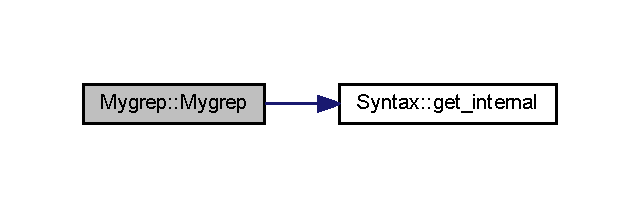
\includegraphics[width=307pt]{class_mygrep_aa2d9dfde7904f2232e6327249f4cd295_cgraph}
\end{center}
\end{figure}




\subsubsection{Методы}
\hypertarget{class_mygrep_a43b5b9e7e2d0ccbee7f5ec0115f53952}{}\index{Mygrep@{Mygrep}!alternate@{alternate}}
\index{alternate@{alternate}!Mygrep@{Mygrep}}
\paragraph[{alternate()}]{\setlength{\rightskip}{0pt plus 5cm}bool Mygrep\+::alternate (
\begin{DoxyParamCaption}
{}
\end{DoxyParamCaption}
)\hspace{0.3cm}{\ttfamily [private]}}\label{class_mygrep_a43b5b9e7e2d0ccbee7f5ec0115f53952}


Перечисление 

Выполняет проверку соответствия входной строки одному из двух выражений-\/операндов \begin{DoxyReturn}{Возвращает}
true, если соответствует одному из выражений, false, если ни одному из выражений не соответствует 
\end{DoxyReturn}


Граф вызовов\+:
\nopagebreak
\begin{figure}[H]
\begin{center}
\leavevmode
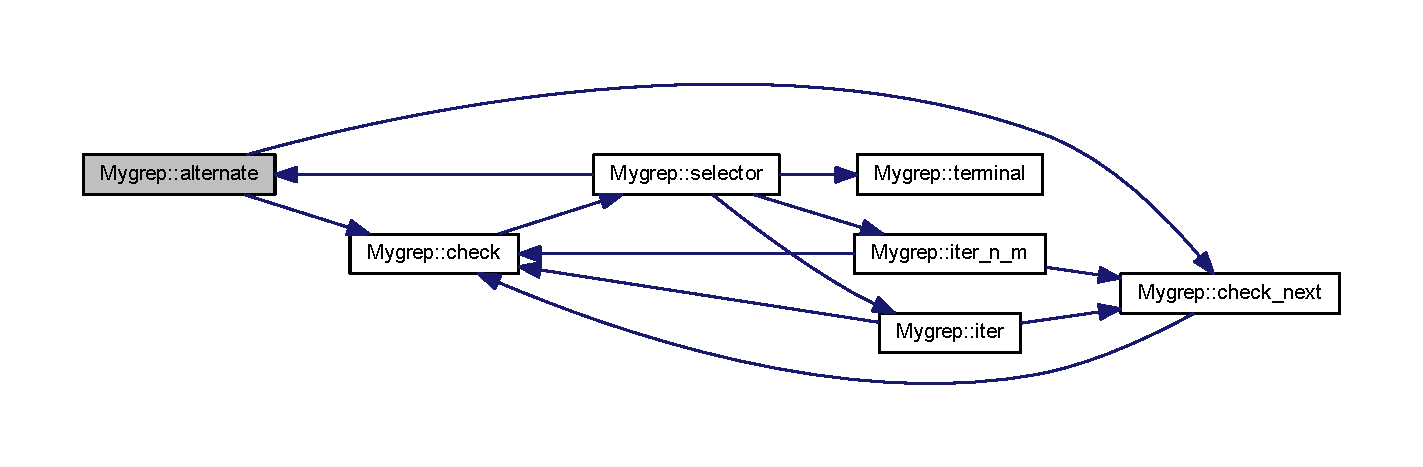
\includegraphics[width=350pt]{class_mygrep_a43b5b9e7e2d0ccbee7f5ec0115f53952_cgraph}
\end{center}
\end{figure}


\hypertarget{class_mygrep_a17b4256c97b2e7e875d50bdc9985ef51}{}\index{Mygrep@{Mygrep}!check@{check}}
\index{check@{check}!Mygrep@{Mygrep}}
\paragraph[{check(const string \&s, bool forsearch=false)}]{\setlength{\rightskip}{0pt plus 5cm}bool Mygrep\+::check (
\begin{DoxyParamCaption}
\item[{const string \&}]{s, }
\item[{bool}]{forsearch = {\ttfamily false}}
\end{DoxyParamCaption}
)}\label{class_mygrep_a17b4256c97b2e7e875d50bdc9985ef51}


Функция сравнения с регулярным выражением 

Проверяет, соответствует ли строка регулярному выражению


\begin{DoxyParams}[1]{Аргументы}
\mbox{\tt in}  & {\em s} & Строка для проверки \\
\hline
\mbox{\tt in}  & {\em forsearch} & Признак того, что проверка выполняется для функции search \\
\hline
\end{DoxyParams}
\begin{DoxyReturn}{Возвращает}
true, если строка соответствует регулярному выражению, false — иначе 
\end{DoxyReturn}


Граф вызовов\+:
\nopagebreak
\begin{figure}[H]
\begin{center}
\leavevmode
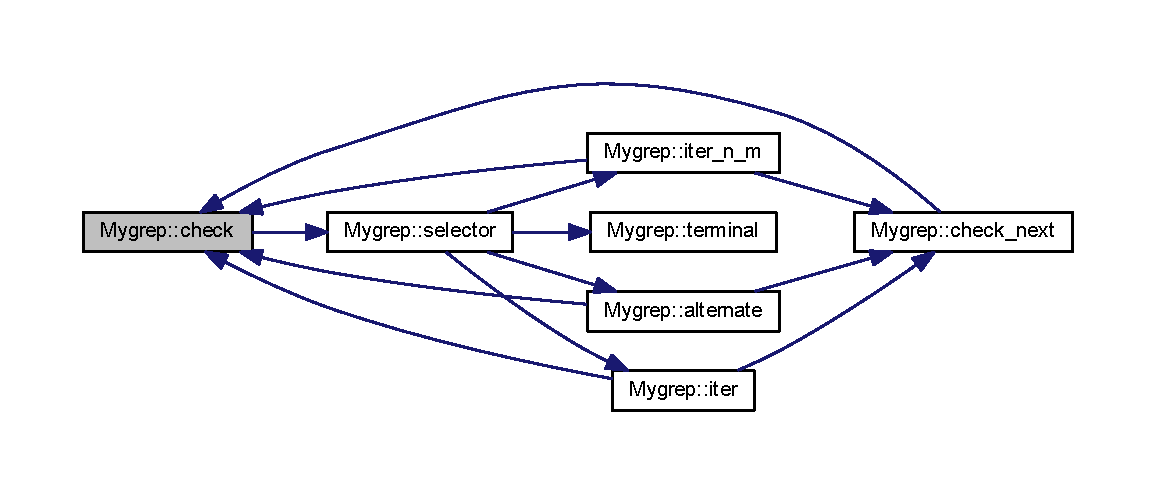
\includegraphics[width=350pt]{class_mygrep_a17b4256c97b2e7e875d50bdc9985ef51_cgraph}
\end{center}
\end{figure}


\hypertarget{class_mygrep_a684ae4e33ce76c8de17b5eadf987afe9}{}\index{Mygrep@{Mygrep}!check@{check}}
\index{check@{check}!Mygrep@{Mygrep}}
\paragraph[{check(vector$<$ Syn\+\_\+lexem $>$ \&v)}]{\setlength{\rightskip}{0pt plus 5cm}bool Mygrep\+::check (
\begin{DoxyParamCaption}
\item[{vector$<$ {\bf Syn\+\_\+lexem} $>$ \&}]{v}
\end{DoxyParamCaption}
)}\label{class_mygrep_a684ae4e33ce76c8de17b5eadf987afe9}


Функция проверки подвыражения 


\begin{DoxyParams}[1]{Аргументы}
\mbox{\tt in}  & {\em v} & Вектор лексем для проверки \\
\hline
\end{DoxyParams}
\begin{DoxyReturn}{Возвращает}
true, если строка соответствует регулярному выражению, false — иначе 
\end{DoxyReturn}


Граф вызовов\+:
\nopagebreak
\begin{figure}[H]
\begin{center}
\leavevmode
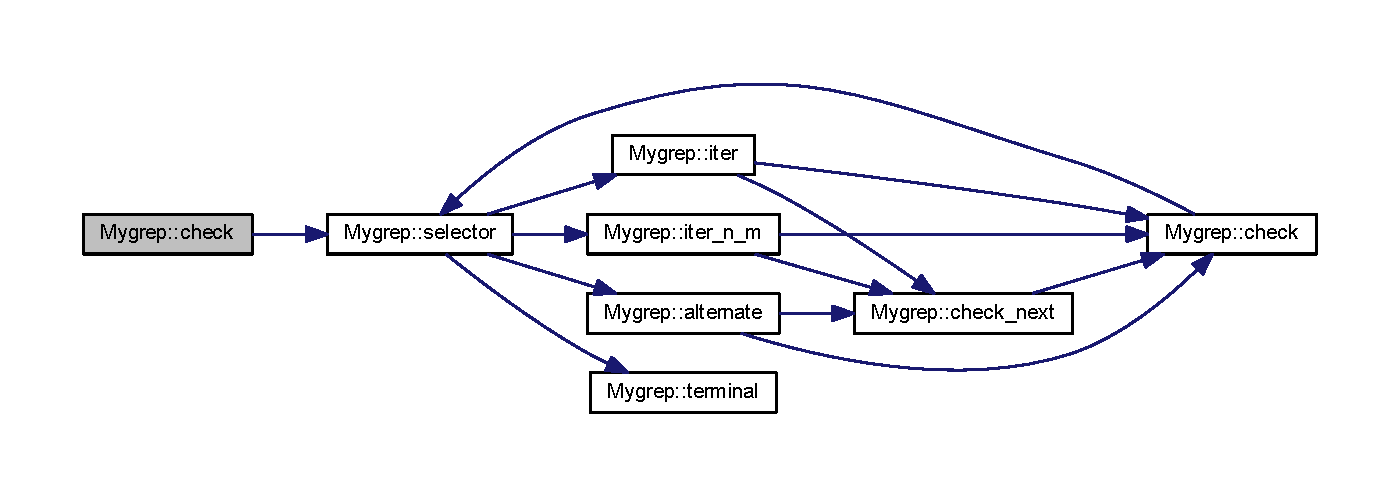
\includegraphics[width=350pt]{class_mygrep_a684ae4e33ce76c8de17b5eadf987afe9_cgraph}
\end{center}
\end{figure}


\hypertarget{class_mygrep_abd79a246feab0fe7548c79b9d887803d}{}\index{Mygrep@{Mygrep}!check\+\_\+next@{check\+\_\+next}}
\index{check\+\_\+next@{check\+\_\+next}!Mygrep@{Mygrep}}
\paragraph[{check\+\_\+next()}]{\setlength{\rightskip}{0pt plus 5cm}bool Mygrep\+::check\+\_\+next (
\begin{DoxyParamCaption}
{}
\end{DoxyParamCaption}
)}\label{class_mygrep_abd79a246feab0fe7548c79b9d887803d}


Проверка следующего 

\begin{DoxyReturn}{Возвращает}
true, если строка соответствует следующим лексемам, false — иначе 
\end{DoxyReturn}


Граф вызовов\+:
\nopagebreak
\begin{figure}[H]
\begin{center}
\leavevmode
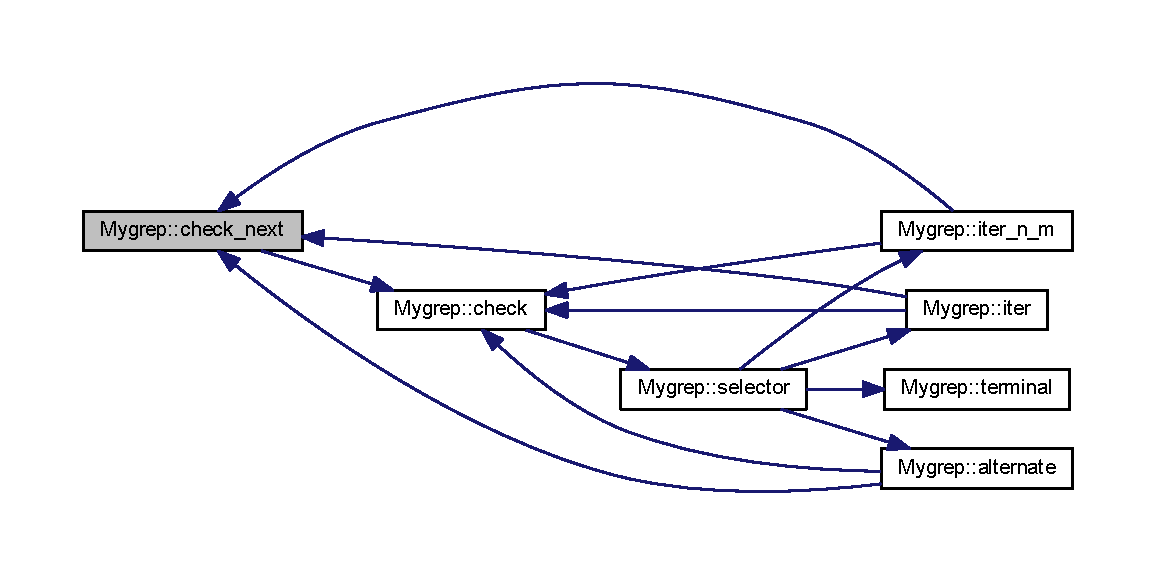
\includegraphics[width=350pt]{class_mygrep_abd79a246feab0fe7548c79b9d887803d_cgraph}
\end{center}
\end{figure}


\hypertarget{class_mygrep_ad893ffcdb0252a2724e5679bf24eeff7}{}\index{Mygrep@{Mygrep}!iter@{iter}}
\index{iter@{iter}!Mygrep@{Mygrep}}
\paragraph[{iter(bool lazy=false)}]{\setlength{\rightskip}{0pt plus 5cm}void Mygrep\+::iter (
\begin{DoxyParamCaption}
\item[{bool}]{lazy = {\ttfamily false}}
\end{DoxyParamCaption}
)\hspace{0.3cm}{\ttfamily [private]}}\label{class_mygrep_ad893ffcdb0252a2724e5679bf24eeff7}


Итерация 

Выполняет итерирацию выражения. В режими поиска подстроки выбирает вариант наибольшего количества итераций 
\begin{DoxyParams}[1]{Аргументы}
\mbox{\tt in}  & {\em lazy} & Признок ленивости иттерации \\
\hline
\end{DoxyParams}


Граф вызовов\+:
\nopagebreak
\begin{figure}[H]
\begin{center}
\leavevmode
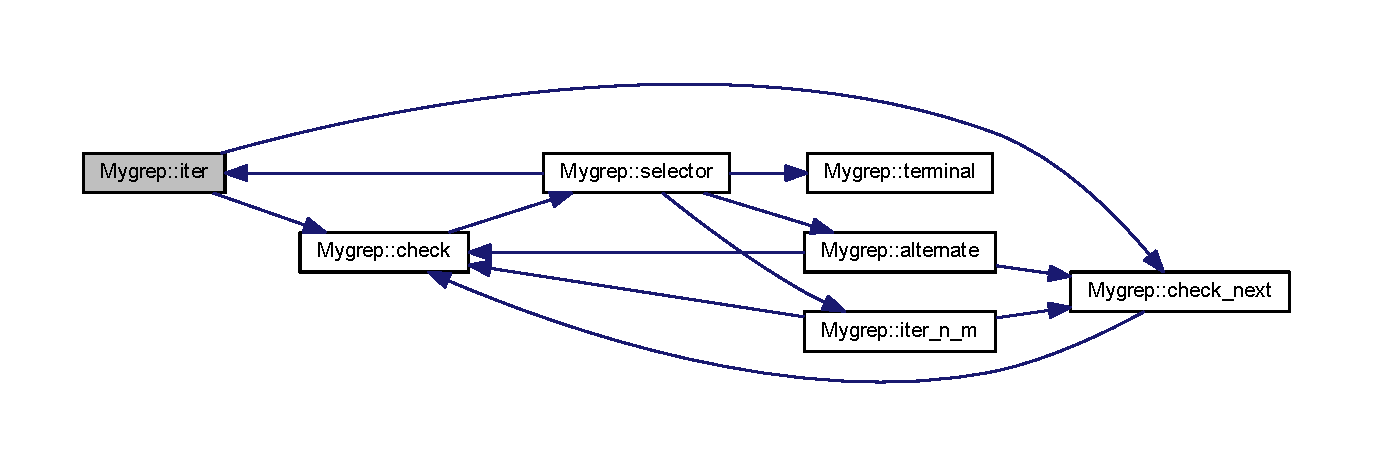
\includegraphics[width=350pt]{class_mygrep_ad893ffcdb0252a2724e5679bf24eeff7_cgraph}
\end{center}
\end{figure}


\hypertarget{class_mygrep_ac52eb295fdae462e39016b0e69bd75bc}{}\index{Mygrep@{Mygrep}!iter\+\_\+n\+\_\+m@{iter\+\_\+n\+\_\+m}}
\index{iter\+\_\+n\+\_\+m@{iter\+\_\+n\+\_\+m}!Mygrep@{Mygrep}}
\paragraph[{iter\+\_\+n\+\_\+m(int n, int m)}]{\setlength{\rightskip}{0pt plus 5cm}bool Mygrep\+::iter\+\_\+n\+\_\+m (
\begin{DoxyParamCaption}
\item[{int}]{n, }
\item[{int}]{m}
\end{DoxyParamCaption}
)\hspace{0.3cm}{\ttfamily [private]}}\label{class_mygrep_ac52eb295fdae462e39016b0e69bd75bc}


Итерация от n до m раз 

Выполняет проверку наличия выражения n раз и выполняет итерацию дополнительно до, возможно, m-\/того раза \begin{DoxyReturn}{Возвращает}
true, если выражение повторяется хотя бы n раз, false — иначе 
\end{DoxyReturn}


Граф вызовов\+:
\nopagebreak
\begin{figure}[H]
\begin{center}
\leavevmode
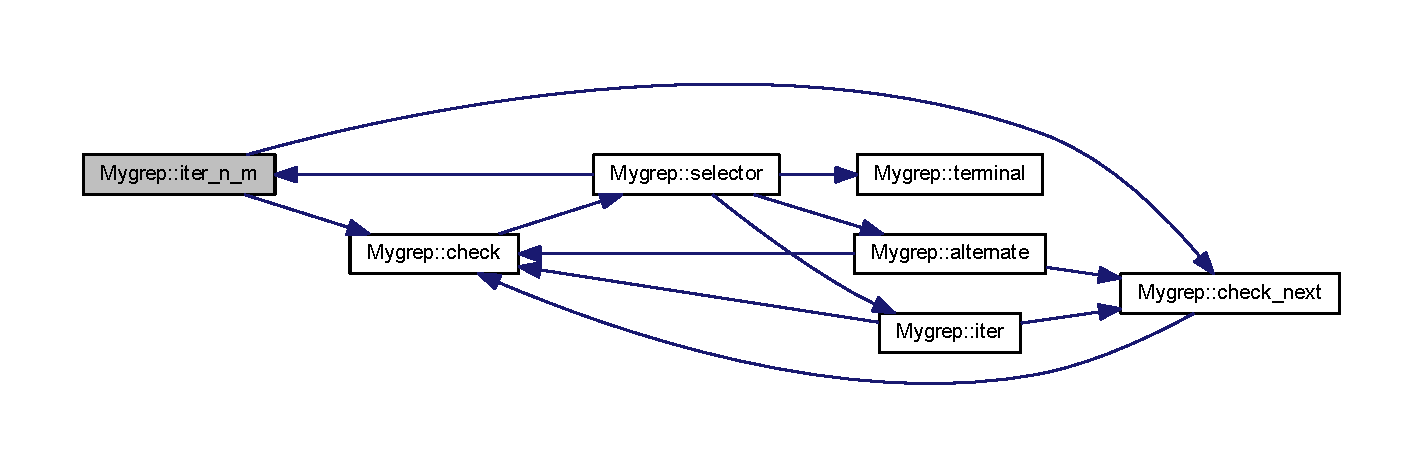
\includegraphics[width=350pt]{class_mygrep_ac52eb295fdae462e39016b0e69bd75bc_cgraph}
\end{center}
\end{figure}


\hypertarget{class_mygrep_a3e4671ac445156bbbcd4f685d61871a5}{}\index{Mygrep@{Mygrep}!search@{search}}
\index{search@{search}!Mygrep@{Mygrep}}
\paragraph[{search(const string \&s)}]{\setlength{\rightskip}{0pt plus 5cm}string Mygrep\+::search (
\begin{DoxyParamCaption}
\item[{const string \&}]{s}
\end{DoxyParamCaption}
)}\label{class_mygrep_a3e4671ac445156bbbcd4f685d61871a5}


Функция поиска подстроки, соответствующей регулярному выражению 

Ищет первое вхождение подстроки, соответствующей регулярному выражению


\begin{DoxyParams}[1]{Аргументы}
\mbox{\tt in}  & {\em s} & Строка для поиска \\
\hline
\end{DoxyParams}
\begin{DoxyReturn}{Возвращает}
Возвращает подстроку, соответствующую регулярному выражению, либо \char`\"{} \char`\"{} (пробел), если подстрока не найдена 
\end{DoxyReturn}


Граф вызовов\+:
\nopagebreak
\begin{figure}[H]
\begin{center}
\leavevmode
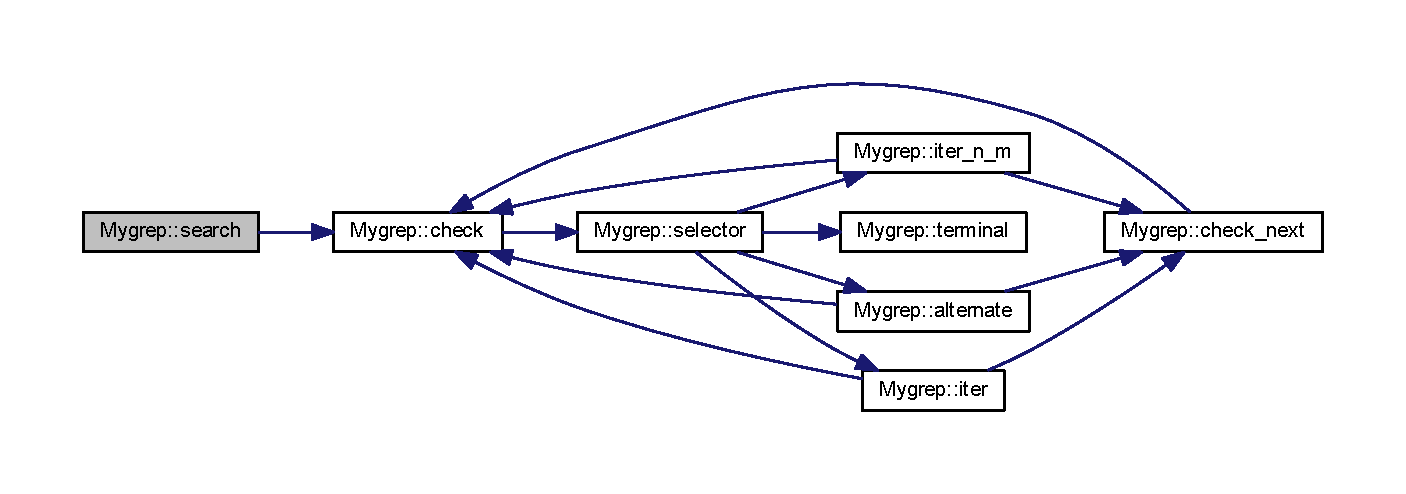
\includegraphics[width=350pt]{class_mygrep_a3e4671ac445156bbbcd4f685d61871a5_cgraph}
\end{center}
\end{figure}


\hypertarget{class_mygrep_ac4293787424bbfe7be6d2585a5f40e9f}{}\index{Mygrep@{Mygrep}!selector@{selector}}
\index{selector@{selector}!Mygrep@{Mygrep}}
\paragraph[{selector()}]{\setlength{\rightskip}{0pt plus 5cm}bool Mygrep\+::selector (
\begin{DoxyParamCaption}
{}
\end{DoxyParamCaption}
)\hspace{0.3cm}{\ttfamily [private]}}\label{class_mygrep_ac4293787424bbfe7be6d2585a5f40e9f}


Функция выбора операции 

Вызывает функцию, соответствующую текущей лексеме \begin{DoxyReturn}{Возвращает}
Возвращает значение вызванной ей функции либо true, если вызывалась неограниченная итерация 
\end{DoxyReturn}


Граф вызовов\+:
\nopagebreak
\begin{figure}[H]
\begin{center}
\leavevmode
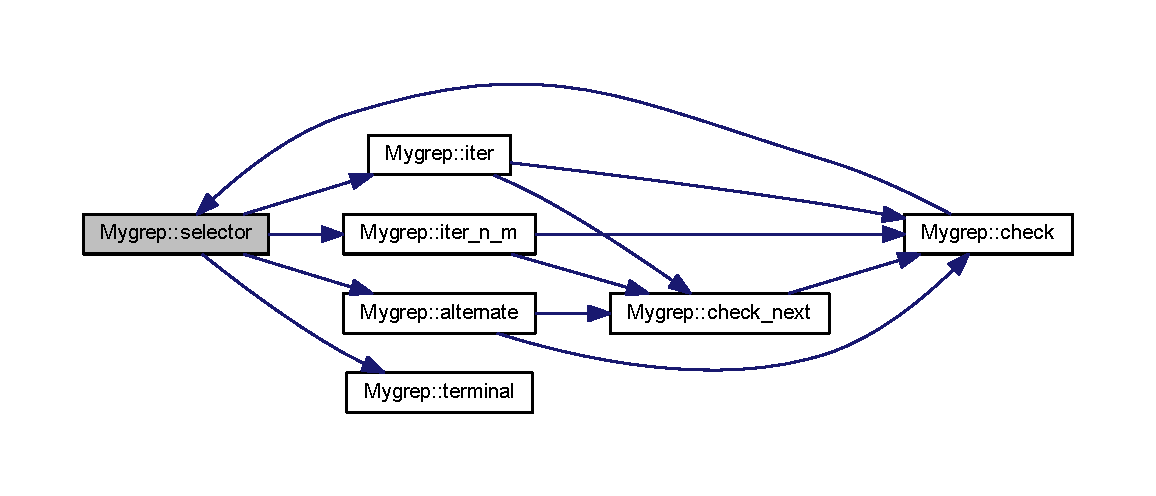
\includegraphics[width=350pt]{class_mygrep_ac4293787424bbfe7be6d2585a5f40e9f_cgraph}
\end{center}
\end{figure}


\hypertarget{class_mygrep_a0e3ee4dc08c04520c4b2af313cf6f9a3}{}\index{Mygrep@{Mygrep}!terminal@{terminal}}
\index{terminal@{terminal}!Mygrep@{Mygrep}}
\paragraph[{terminal()}]{\setlength{\rightskip}{0pt plus 5cm}bool Mygrep\+::terminal (
\begin{DoxyParamCaption}
{}
\end{DoxyParamCaption}
)\hspace{0.3cm}{\ttfamily [private]}}\label{class_mygrep_a0e3ee4dc08c04520c4b2af313cf6f9a3}


Терминал 

Выполняет проверку наличия необходимой терминальной последовательности на позиции входной строки, анализируемой в данный момент \begin{DoxyReturn}{Возвращает}
true, если терминальная последовательность обнаружена, false — иначе 
\end{DoxyReturn}


Объявления и описания членов классов находятся в файлах\+:\begin{DoxyCompactItemize}
\item 
\hyperlink{mygrep_8h}{mygrep.\+h}\item 
\hyperlink{mygrep_8cpp}{mygrep.\+cpp}\end{DoxyCompactItemize}

\hypertarget{class_syn__lexem}{}\subsection{Класс Syn\+\_\+lexem}
\label{class_syn__lexem}\index{Syn\+\_\+lexem@{Syn\+\_\+lexem}}


Синтаксические лексемы  




{\ttfamily \#include $<$syntax.\+h$>$}

\subsubsection*{Закрытые члены}
\begin{DoxyCompactItemize}
\item 
\hyperlink{class_syn__lexem_a41cbc6daa60c91a689593635f4ab7e68}{Syn\+\_\+lexem} (\hyperlink{class_lexem}{Lexem} \&lexem)
\item 
\hyperlink{class_syn__lexem_a4c905eacfd6896facc415ab1e66dd848}{Syn\+\_\+lexem} (int \hyperlink{class_syn__lexem_a05e633f5cc7073402b8324a28fba6c54}{param2}, vector$<$ \hyperlink{class_syn__lexem}{Syn\+\_\+lexem} $>$ operand)
\item 
void \hyperlink{class_syn__lexem_aeeae755d5f4283c36fd405fa1ba997d6}{print} ()
\end{DoxyCompactItemize}
\subsubsection*{Закрытые данные}
\begin{DoxyCompactItemize}
\item 
\hypertarget{class_syn__lexem_a8a7ffdf228251a8f3d804ac9b03c5122}{}\hyperlink{class_lexem_af335177220e991d190a36fabef7ecbf4}{Lexem\+::lexem\+\_\+types} \hyperlink{class_syn__lexem_a8a7ffdf228251a8f3d804ac9b03c5122}{type}\label{class_syn__lexem_a8a7ffdf228251a8f3d804ac9b03c5122}

\begin{DoxyCompactList}\small\item\em Тип лексемы \end{DoxyCompactList}\item 
\hypertarget{class_syn__lexem_a60715814abcd1fe72ba3583eed998ea3}{}string \hyperlink{class_syn__lexem_a60715814abcd1fe72ba3583eed998ea3}{terminal} = \char`\"{}\char`\"{}\label{class_syn__lexem_a60715814abcd1fe72ba3583eed998ea3}

\begin{DoxyCompactList}\small\item\em Терминальная цепочка \end{DoxyCompactList}\item 
\hypertarget{class_syn__lexem_a514891b78ea7e818210be401075371aa}{}int \hyperlink{class_syn__lexem_a514891b78ea7e818210be401075371aa}{param1} = 0\label{class_syn__lexem_a514891b78ea7e818210be401075371aa}

\begin{DoxyCompactList}\small\item\em Первый параметр лексемы \end{DoxyCompactList}\item 
\hypertarget{class_syn__lexem_a05e633f5cc7073402b8324a28fba6c54}{}int \hyperlink{class_syn__lexem_a05e633f5cc7073402b8324a28fba6c54}{param2} = 0\label{class_syn__lexem_a05e633f5cc7073402b8324a28fba6c54}

\begin{DoxyCompactList}\small\item\em Второй параметр лексемы \end{DoxyCompactList}\item 
\hypertarget{class_syn__lexem_ac1273e1e14c1f7912bf6ca79e9ce3a2b}{}vector$<$ \hyperlink{class_syn__lexem}{Syn\+\_\+lexem} $>$ \hyperlink{class_syn__lexem_ac1273e1e14c1f7912bf6ca79e9ce3a2b}{operand1}\label{class_syn__lexem_ac1273e1e14c1f7912bf6ca79e9ce3a2b}

\begin{DoxyCompactList}\small\item\em Первый операнд \end{DoxyCompactList}\item 
\hypertarget{class_syn__lexem_a2785b2c17862062c1b0413f6fd8a5dbd}{}vector$<$ \hyperlink{class_syn__lexem}{Syn\+\_\+lexem} $>$ \hyperlink{class_syn__lexem_a2785b2c17862062c1b0413f6fd8a5dbd}{operand2}\label{class_syn__lexem_a2785b2c17862062c1b0413f6fd8a5dbd}

\begin{DoxyCompactList}\small\item\em Второй операнд \end{DoxyCompactList}\end{DoxyCompactItemize}
\subsubsection*{Друзья}
\begin{DoxyCompactItemize}
\item 
\hypertarget{class_syn__lexem_a13fb68a36cac69480f7fd4b3900594f9}{}class {\bfseries Syntax}\label{class_syn__lexem_a13fb68a36cac69480f7fd4b3900594f9}

\item 
\hypertarget{class_syn__lexem_a90fdb1ff12233c504810e346b5f6e49f}{}class {\bfseries Mygrep}\label{class_syn__lexem_a90fdb1ff12233c504810e346b5f6e49f}

\end{DoxyCompactItemize}


\subsubsection{Подробное описание}
Синтаксические лексемы 

\subsubsection{Конструктор(ы)}
\hypertarget{class_syn__lexem_a41cbc6daa60c91a689593635f4ab7e68}{}\index{Syn\+\_\+lexem@{Syn\+\_\+lexem}!Syn\+\_\+lexem@{Syn\+\_\+lexem}}
\index{Syn\+\_\+lexem@{Syn\+\_\+lexem}!Syn\+\_\+lexem@{Syn\+\_\+lexem}}
\paragraph[{Syn\+\_\+lexem(\+Lexem \&lexem)}]{\setlength{\rightskip}{0pt plus 5cm}Syn\+\_\+lexem\+::\+Syn\+\_\+lexem (
\begin{DoxyParamCaption}
\item[{{\bf Lexem} \&}]{lexem}
\end{DoxyParamCaption}
)\hspace{0.3cm}{\ttfamily [private]}}\label{class_syn__lexem_a41cbc6daa60c91a689593635f4ab7e68}
Конструктор построения синтаксической лексемы по обычной 
\begin{DoxyParams}[1]{Аргументы}
\mbox{\tt in}  & {\em lexem} & Обычная лексема \\
\hline
\end{DoxyParams}
\hypertarget{class_syn__lexem_a4c905eacfd6896facc415ab1e66dd848}{}\index{Syn\+\_\+lexem@{Syn\+\_\+lexem}!Syn\+\_\+lexem@{Syn\+\_\+lexem}}
\index{Syn\+\_\+lexem@{Syn\+\_\+lexem}!Syn\+\_\+lexem@{Syn\+\_\+lexem}}
\paragraph[{Syn\+\_\+lexem(int param2, vector$<$ Syn\+\_\+lexem $>$ operand)}]{\setlength{\rightskip}{0pt plus 5cm}Syn\+\_\+lexem\+::\+Syn\+\_\+lexem (
\begin{DoxyParamCaption}
\item[{int}]{param2, }
\item[{vector$<$ {\bf Syn\+\_\+lexem} $>$}]{operand}
\end{DoxyParamCaption}
)\hspace{0.3cm}{\ttfamily [private]}}\label{class_syn__lexem_a4c905eacfd6896facc415ab1e66dd848}
Конструктор лексемы итерация от 0 до param2 раз 
\begin{DoxyParams}[1]{Аргументы}
\mbox{\tt in}  & {\em param2} & Максимальное количество итераций \\
\hline
\mbox{\tt in}  & {\em operand} & Операнд итерации \\
\hline
\end{DoxyParams}


\subsubsection{Методы}
\hypertarget{class_syn__lexem_aeeae755d5f4283c36fd405fa1ba997d6}{}\index{Syn\+\_\+lexem@{Syn\+\_\+lexem}!print@{print}}
\index{print@{print}!Syn\+\_\+lexem@{Syn\+\_\+lexem}}
\paragraph[{print()}]{\setlength{\rightskip}{0pt plus 5cm}void Syn\+\_\+lexem\+::print (
\begin{DoxyParamCaption}
{}
\end{DoxyParamCaption}
)\hspace{0.3cm}{\ttfamily [private]}}\label{class_syn__lexem_aeeae755d5f4283c36fd405fa1ba997d6}
Печать лексемы 

Объявления и описания членов классов находятся в файлах\+:\begin{DoxyCompactItemize}
\item 
\hyperlink{syntax_8h}{syntax.\+h}\item 
\hyperlink{syntax_8cpp}{syntax.\+cpp}\end{DoxyCompactItemize}

\hypertarget{class_syntax}{}\subsection{Класс Syntax}
\label{class_syntax}\index{Syntax@{Syntax}}


Синтаксический анализатор  




{\ttfamily \#include $<$syntax.\+h$>$}



Граф связей класса Syntax\+:
\nopagebreak
\begin{figure}[H]
\begin{center}
\leavevmode
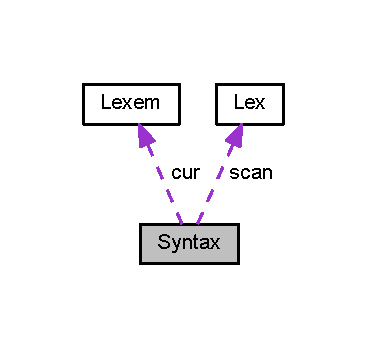
\includegraphics[width=176pt]{class_syntax__coll__graph}
\end{center}
\end{figure}
\subsubsection*{Закрытые члены}
\begin{DoxyCompactItemize}
\item 
\hypertarget{class_syntax_a5139d8fddfa05e199bf12b8ef7bd3620}{}void \hyperlink{class_syntax_a5139d8fddfa05e199bf12b8ef7bd3620}{gl} ()\label{class_syntax_a5139d8fddfa05e199bf12b8ef7bd3620}

\begin{DoxyCompactList}\small\item\em Функция, получающая из лексического анализатора очередную лексему и записывающая её в переменную cur. \end{DoxyCompactList}\item 
\hyperlink{class_syntax_a52bc44b52e3dceea48a1e71f65d5e3cf}{Syntax} (const string \&reg)
\begin{DoxyCompactList}\small\item\em Конструктор от строки с регулярным выражением. \end{DoxyCompactList}\item 
vector$<$ \hyperlink{class_syn__lexem}{Syn\+\_\+lexem} $>$ \hyperlink{class_syntax_a61442ccace7e6d58205cc2988bd5391b}{get\+\_\+internal} ()
\begin{DoxyCompactList}\small\item\em Функция, возвращающая внутреннее представление \end{DoxyCompactList}\end{DoxyCompactItemize}
\begin{Indent}{\bf Функции РС-\/метода}\par
\begin{DoxyCompactItemize}
\item 
void \hyperlink{class_syntax_af5d09263aadaa0b9a264ebf436beb9e8}{S} ()
\begin{DoxyCompactList}\small\item\em Начальное состояние \end{DoxyCompactList}\item 
vector$<$ \hyperlink{class_syn__lexem}{Syn\+\_\+lexem} $>$ \hyperlink{class_syntax_ad3bf45fadc4d20146f0a6c85d970d714}{S1} (bool concat=false)
\begin{DoxyCompactList}\small\item\em Основное состояние \end{DoxyCompactList}\item 
vector$<$ \hyperlink{class_syn__lexem}{Syn\+\_\+lexem} $>$ \hyperlink{class_syntax_a4ed2d9c690da119299e6e74fc9332f16}{O} (vector$<$ \hyperlink{class_syn__lexem}{Syn\+\_\+lexem} $>$ \&operand)
\begin{DoxyCompactList}\small\item\em Состояние поиска унарного оператора \end{DoxyCompactList}\end{DoxyCompactItemize}
\end{Indent}
\subsubsection*{Закрытые данные}
\begin{DoxyCompactItemize}
\item 
\hypertarget{class_syntax_afa60cc2342d74dbdbb8679ee1677b8e1}{}\hyperlink{class_lex}{Lex} \hyperlink{class_syntax_afa60cc2342d74dbdbb8679ee1677b8e1}{scan}\label{class_syntax_afa60cc2342d74dbdbb8679ee1677b8e1}

\begin{DoxyCompactList}\small\item\em Лексический анализатор \end{DoxyCompactList}\item 
\hypertarget{class_syntax_a18d0feb830951877fef2692ea77f931b}{}\hyperlink{class_lexem}{Lexem} \hyperlink{class_syntax_a18d0feb830951877fef2692ea77f931b}{cur}\label{class_syntax_a18d0feb830951877fef2692ea77f931b}

\begin{DoxyCompactList}\small\item\em Текущая лексема \end{DoxyCompactList}\item 
\hypertarget{class_syntax_a2337e4b3bc2ff71bddf65ca7461c012c}{}int \hyperlink{class_syntax_a2337e4b3bc2ff71bddf65ca7461c012c}{countbrace} = 0\label{class_syntax_a2337e4b3bc2ff71bddf65ca7461c012c}

\begin{DoxyCompactList}\small\item\em Счётчик скобок \end{DoxyCompactList}\item 
\hypertarget{class_syntax_ae2ce745407fa89c47376e82bc208162e}{}vector$<$ \hyperlink{class_syn__lexem}{Syn\+\_\+lexem} $>$ \hyperlink{class_syntax_ae2ce745407fa89c47376e82bc208162e}{internal}\label{class_syntax_ae2ce745407fa89c47376e82bc208162e}

\begin{DoxyCompactList}\small\item\em Внутреннее представление выражения \end{DoxyCompactList}\end{DoxyCompactItemize}
\subsubsection*{Друзья}
\begin{DoxyCompactItemize}
\item 
\hypertarget{class_syntax_a90fdb1ff12233c504810e346b5f6e49f}{}class {\bfseries Mygrep}\label{class_syntax_a90fdb1ff12233c504810e346b5f6e49f}

\end{DoxyCompactItemize}


\subsubsection{Подробное описание}
Синтаксический анализатор 

Синтаксический анализатор проверяет последовательность типизированных лексем на соответствии грамматике языка регулярных выражений и переводит последотельность во внутреннее представление (последовательность синтаксических лексем) 

\subsubsection{Конструктор(ы)}
\hypertarget{class_syntax_a52bc44b52e3dceea48a1e71f65d5e3cf}{}\index{Syntax@{Syntax}!Syntax@{Syntax}}
\index{Syntax@{Syntax}!Syntax@{Syntax}}
\paragraph[{Syntax(const string \&reg)}]{\setlength{\rightskip}{0pt plus 5cm}Syntax\+::\+Syntax (
\begin{DoxyParamCaption}
\item[{const string \&}]{reg}
\end{DoxyParamCaption}
)\hspace{0.3cm}{\ttfamily [explicit]}, {\ttfamily [private]}}\label{class_syntax_a52bc44b52e3dceea48a1e71f65d5e3cf}


Конструктор от строки с регулярным выражением. 

Сделан явным, поскольку неясен смысл выражения вида \hyperlink{class_syntax}{Syntax} c = \char`\"{}a$\ast$\char`\"{}; 

Граф вызовов\+:
\nopagebreak
\begin{figure}[H]
\begin{center}
\leavevmode
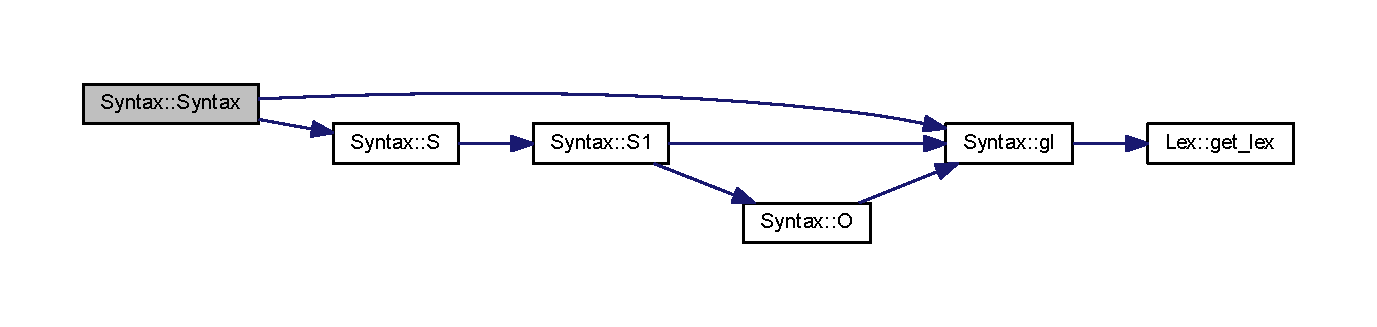
\includegraphics[width=350pt]{class_syntax_a52bc44b52e3dceea48a1e71f65d5e3cf_cgraph}
\end{center}
\end{figure}




\subsubsection{Методы}
\hypertarget{class_syntax_a61442ccace7e6d58205cc2988bd5391b}{}\index{Syntax@{Syntax}!get\+\_\+internal@{get\+\_\+internal}}
\index{get\+\_\+internal@{get\+\_\+internal}!Syntax@{Syntax}}
\paragraph[{get\+\_\+internal()}]{\setlength{\rightskip}{0pt plus 5cm}vector$<$ {\bf Syn\+\_\+lexem} $>$ Syntax\+::get\+\_\+internal (
\begin{DoxyParamCaption}
{}
\end{DoxyParamCaption}
)\hspace{0.3cm}{\ttfamily [private]}}\label{class_syntax_a61442ccace7e6d58205cc2988bd5391b}


Функция, возвращающая внутреннее представление 

\begin{DoxyReturn}{Возвращает}
Возвращают сгенерированное внутреннего представления выражения 
\end{DoxyReturn}
\hypertarget{class_syntax_a4ed2d9c690da119299e6e74fc9332f16}{}\index{Syntax@{Syntax}!O@{O}}
\index{O@{O}!Syntax@{Syntax}}
\paragraph[{O(vector$<$ Syn\+\_\+lexem $>$ \&operand)}]{\setlength{\rightskip}{0pt plus 5cm}vector$<$ {\bf Syn\+\_\+lexem} $>$ Syntax\+::\+O (
\begin{DoxyParamCaption}
\item[{vector$<$ {\bf Syn\+\_\+lexem} $>$ \&}]{operand}
\end{DoxyParamCaption}
)\hspace{0.3cm}{\ttfamily [private]}}\label{class_syntax_a4ed2d9c690da119299e6e74fc9332f16}


Состояние поиска унарного оператора 

\begin{DoxyReturn}{Возвращает}
Возвращают сгенерированную подпоследовательность внутреннего представления 
\end{DoxyReturn}


Граф вызовов\+:
\nopagebreak
\begin{figure}[H]
\begin{center}
\leavevmode
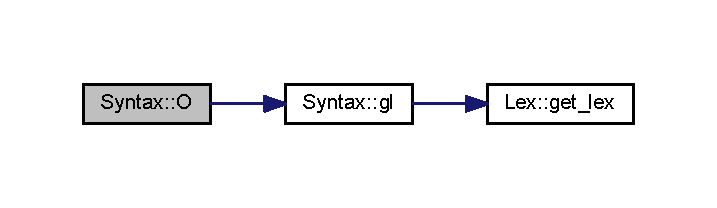
\includegraphics[width=344pt]{class_syntax_a4ed2d9c690da119299e6e74fc9332f16_cgraph}
\end{center}
\end{figure}


\hypertarget{class_syntax_af5d09263aadaa0b9a264ebf436beb9e8}{}\index{Syntax@{Syntax}!S@{S}}
\index{S@{S}!Syntax@{Syntax}}
\paragraph[{S()}]{\setlength{\rightskip}{0pt plus 5cm}void Syntax\+::\+S (
\begin{DoxyParamCaption}
{}
\end{DoxyParamCaption}
)\hspace{0.3cm}{\ttfamily [private]}}\label{class_syntax_af5d09263aadaa0b9a264ebf436beb9e8}


Начальное состояние 

Либо обнаруживает пустую последовательность, либо переходит в состояние S1 

Граф вызовов\+:
\nopagebreak
\begin{figure}[H]
\begin{center}
\leavevmode
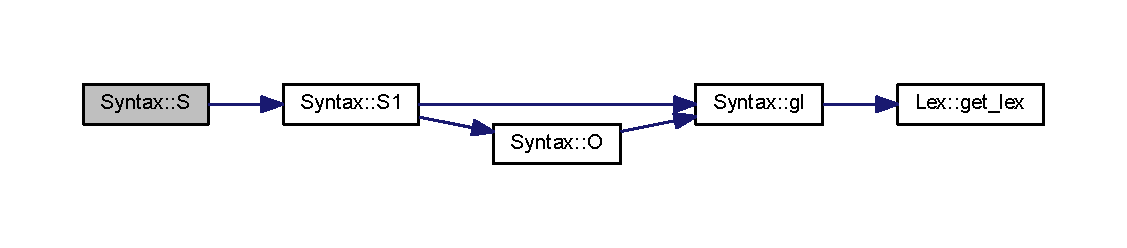
\includegraphics[width=350pt]{class_syntax_af5d09263aadaa0b9a264ebf436beb9e8_cgraph}
\end{center}
\end{figure}


\hypertarget{class_syntax_ad3bf45fadc4d20146f0a6c85d970d714}{}\index{Syntax@{Syntax}!S1@{S1}}
\index{S1@{S1}!Syntax@{Syntax}}
\paragraph[{S1(bool concat=false)}]{\setlength{\rightskip}{0pt plus 5cm}vector$<$ {\bf Syn\+\_\+lexem} $>$ Syntax\+::\+S1 (
\begin{DoxyParamCaption}
\item[{bool}]{concat = {\ttfamily false}}
\end{DoxyParamCaption}
)\hspace{0.3cm}{\ttfamily [private]}}\label{class_syntax_ad3bf45fadc4d20146f0a6c85d970d714}


Основное состояние 

\begin{DoxyReturn}{Возвращает}
Возвращают сгенерированную подпоследовательность внутреннего представления 
\end{DoxyReturn}


Граф вызовов\+:
\nopagebreak
\begin{figure}[H]
\begin{center}
\leavevmode
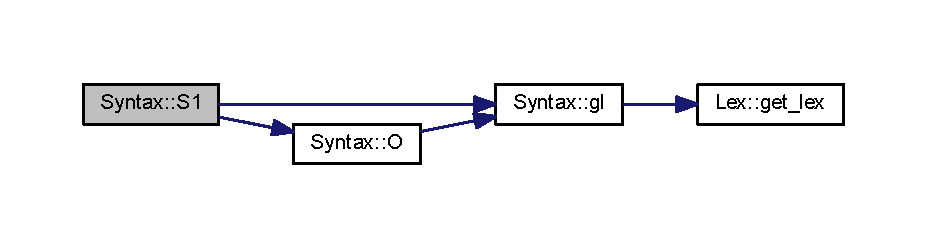
\includegraphics[width=350pt]{class_syntax_ad3bf45fadc4d20146f0a6c85d970d714_cgraph}
\end{center}
\end{figure}




Объявления и описания членов классов находятся в файлах\+:\begin{DoxyCompactItemize}
\item 
\hyperlink{syntax_8h}{syntax.\+h}\item 
\hyperlink{syntax_8cpp}{syntax.\+cpp}\end{DoxyCompactItemize}

\section{Файлы}
\hypertarget{lexic_8cpp}{}\subsection{Файл lexic.\+cpp}
\label{lexic_8cpp}\index{lexic.\+cpp@{lexic.\+cpp}}


Файл с реализацией лексического анализатора  


{\ttfamily \#include $<$vector$>$}\\*
{\ttfamily \#include $<$string$>$}\\*
{\ttfamily \#include $<$iostream$>$}\\*
{\ttfamily \#include $<$stdexcept$>$}\\*
{\ttfamily \#include $<$cctype$>$}\\*
{\ttfamily \#include \char`\"{}lexic.\+h\char`\"{}}\\*
Граф включаемых заголовочных файлов для lexic.\+cpp\+:
\nopagebreak
\begin{figure}[H]
\begin{center}
\leavevmode
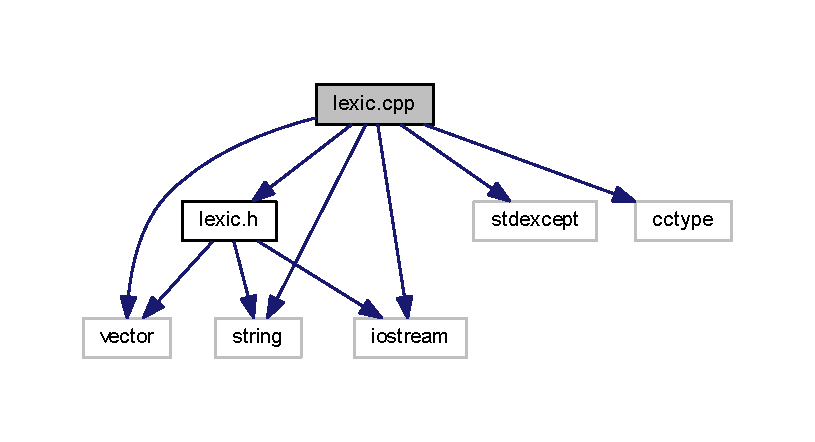
\includegraphics[width=350pt]{lexic_8cpp__incl}
\end{center}
\end{figure}


\subsubsection{Подробное описание}
Файл с реализацией лексического анализатора 

Данный файл содержит в себе реализацию всех методов классов \hyperlink{class_lex}{Lex} и \hyperlink{class_lexem}{Lexem} 
\hypertarget{lexic_8h}{}\subsection{Файл lexic.\+h}
\label{lexic_8h}\index{lexic.\+h@{lexic.\+h}}


Заголовочный файл лексического анализатора  


{\ttfamily \#include $<$iostream$>$}\\*
{\ttfamily \#include $<$vector$>$}\\*
{\ttfamily \#include $<$string$>$}\\*
Граф включаемых заголовочных файлов для lexic.\+h\+:
\nopagebreak
\begin{figure}[H]
\begin{center}
\leavevmode
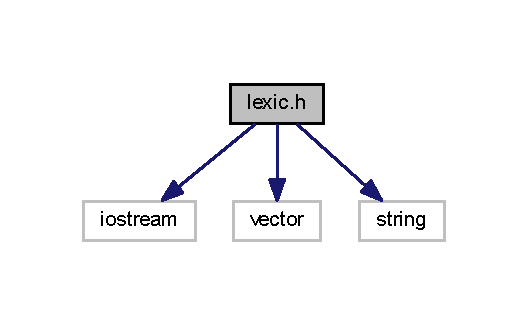
\includegraphics[width=254pt]{lexic_8h__incl}
\end{center}
\end{figure}
Граф файлов, в которые включается этот файл\+:
\nopagebreak
\begin{figure}[H]
\begin{center}
\leavevmode
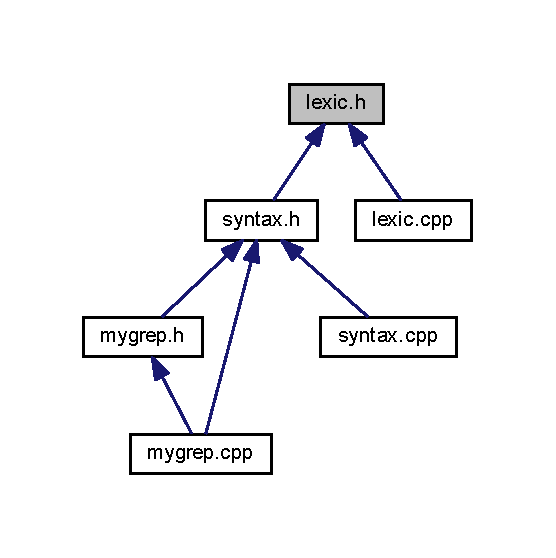
\includegraphics[width=267pt]{lexic_8h__dep__incl}
\end{center}
\end{figure}
\subsubsection*{Классы}
\begin{DoxyCompactItemize}
\item 
class \hyperlink{class_lexem}{Lexem}
\begin{DoxyCompactList}\small\item\em Класс лексем \end{DoxyCompactList}\item 
class \hyperlink{class_lex}{Lex}
\begin{DoxyCompactList}\small\item\em Лексический анализатор \end{DoxyCompactList}\end{DoxyCompactItemize}


\subsubsection{Подробное описание}
Заголовочный файл лексического анализатора 

Данный файл содержит в себе определения структуры лексем и класса лексического анализатора 
\hypertarget{mygrep_8cpp}{}\subsection{Файл mygrep.\+cpp}
\label{mygrep_8cpp}\index{mygrep.\+cpp@{mygrep.\+cpp}}


Файл с реализацией основного функционала программы  


{\ttfamily \#include \char`\"{}mygrep.\+h\char`\"{}}\\*
{\ttfamily \#include \char`\"{}syntax.\+h\char`\"{}}\\*
{\ttfamily \#include $<$string$>$}\\*
Граф включаемых заголовочных файлов для mygrep.\+cpp\+:
\nopagebreak
\begin{figure}[H]
\begin{center}
\leavevmode
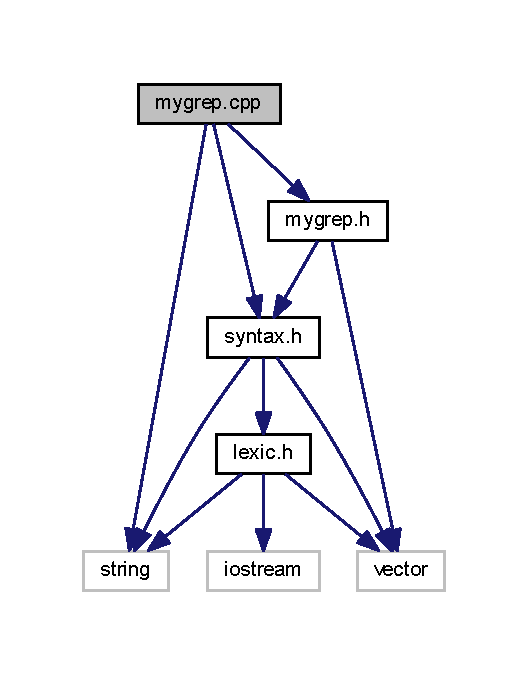
\includegraphics[width=254pt]{mygrep_8cpp__incl}
\end{center}
\end{figure}


\subsubsection{Подробное описание}
Файл с реализацией основного функционала программы 

Данный файл содержит в себе реализацию всех методов класса \hyperlink{class_mygrep}{Mygrep} 
\hypertarget{mygrep_8h}{}\subsection{Файл mygrep.\+h}
\label{mygrep_8h}\index{mygrep.\+h@{mygrep.\+h}}


Заголовочный файл пользовательськой части программы  


{\ttfamily \#include \char`\"{}syntax.\+h\char`\"{}}\\*
{\ttfamily \#include $<$vector$>$}\\*
Граф включаемых заголовочных файлов для mygrep.\+h\+:
\nopagebreak
\begin{figure}[H]
\begin{center}
\leavevmode
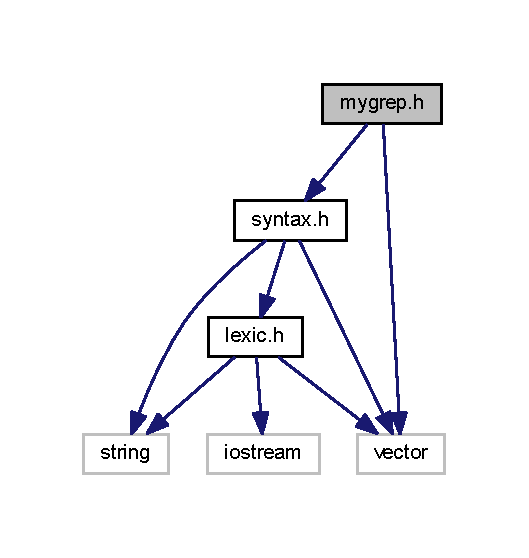
\includegraphics[width=254pt]{mygrep_8h__incl}
\end{center}
\end{figure}
Граф файлов, в которые включается этот файл\+:
\nopagebreak
\begin{figure}[H]
\begin{center}
\leavevmode
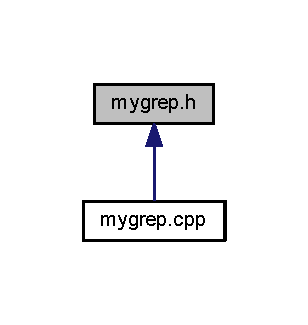
\includegraphics[width=148pt]{mygrep_8h__dep__incl}
\end{center}
\end{figure}
\subsubsection*{Классы}
\begin{DoxyCompactItemize}
\item 
class \hyperlink{class_mygrep}{Mygrep}
\begin{DoxyCompactList}\small\item\em Обработчик регулярных выражений \end{DoxyCompactList}\end{DoxyCompactItemize}


\subsubsection{Подробное описание}
Заголовочный файл пользовательськой части программы 

Данный файл содержит в себе определение класса-\/обработчика регулярных выражений 
\hypertarget{syntax_8cpp}{}\subsection{Файл syntax.\+cpp}
\label{syntax_8cpp}\index{syntax.\+cpp@{syntax.\+cpp}}


Файл с реализацией синтаксического анализатора  


{\ttfamily \#include \char`\"{}syntax.\+h\char`\"{}}\\*
{\ttfamily \#include $<$stdexcept$>$}\\*
Граф включаемых заголовочных файлов для syntax.\+cpp\+:
\nopagebreak
\begin{figure}[H]
\begin{center}
\leavevmode
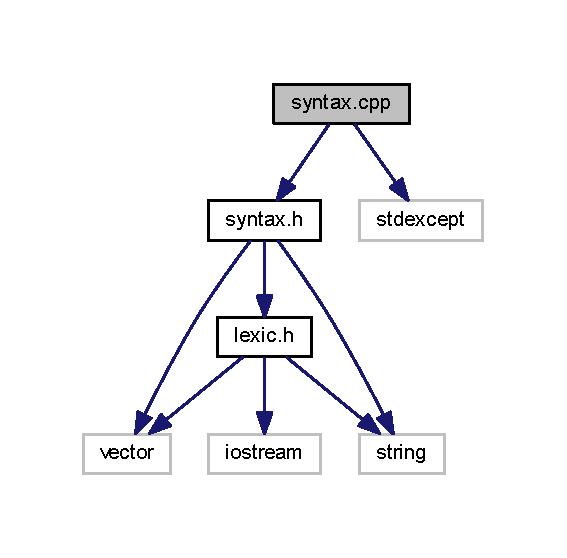
\includegraphics[width=272pt]{syntax_8cpp__incl}
\end{center}
\end{figure}


\subsubsection{Подробное описание}
Файл с реализацией синтаксического анализатора 

Данный файл содержит в себе реализацию всех методов классов \hyperlink{class_syntax}{Syntax} и \hyperlink{class_syn__lexem}{Syn\+\_\+lexem} 
\hypertarget{syntax_8h}{}\subsection{Файл syntax.\+h}
\label{syntax_8h}\index{syntax.\+h@{syntax.\+h}}


Заголовочный файл синтаксического анализатора  


{\ttfamily \#include \char`\"{}lexic.\+h\char`\"{}}\\*
{\ttfamily \#include $<$vector$>$}\\*
{\ttfamily \#include $<$string$>$}\\*
Граф включаемых заголовочных файлов для syntax.\+h\+:
\nopagebreak
\begin{figure}[H]
\begin{center}
\leavevmode
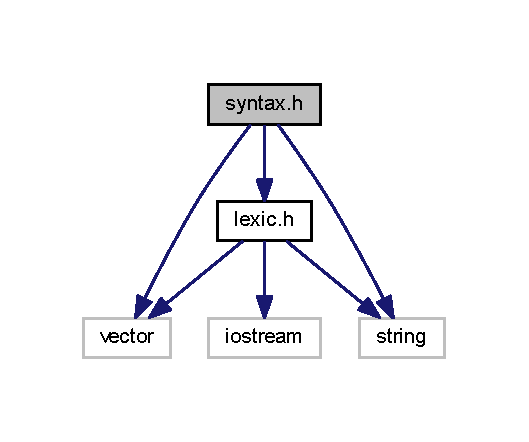
\includegraphics[width=254pt]{syntax_8h__incl}
\end{center}
\end{figure}
Граф файлов, в которые включается этот файл\+:
\nopagebreak
\begin{figure}[H]
\begin{center}
\leavevmode
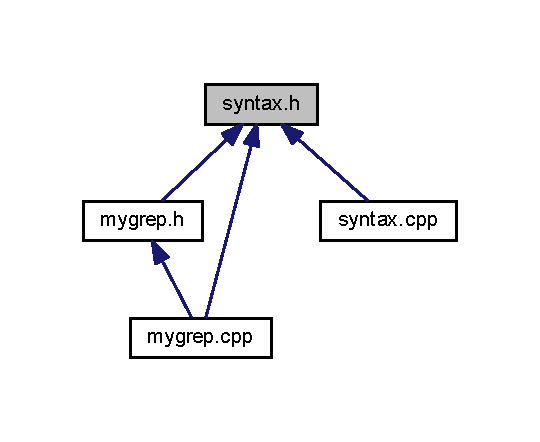
\includegraphics[width=259pt]{syntax_8h__dep__incl}
\end{center}
\end{figure}
\subsubsection*{Классы}
\begin{DoxyCompactItemize}
\item 
class \hyperlink{class_syn__lexem}{Syn\+\_\+lexem}
\begin{DoxyCompactList}\small\item\em Синтаксические лексемы \end{DoxyCompactList}\item 
class \hyperlink{class_syntax}{Syntax}
\begin{DoxyCompactList}\small\item\em Синтаксический анализатор \end{DoxyCompactList}\end{DoxyCompactItemize}


\subsubsection{Подробное описание}
Заголовочный файл синтаксического анализатора 

Данный файл содержит в себе определения класса синтаксического анализатора 
%--- End generated contents ---

% Index
\newpage
\phantomsection
\clearemptydoublepage
\addcontentsline{toc}{section}{Алфавитный указатель}
\printindex

\end{document}
